\chapter{Метод расчета траекторий движения индивидуальных жидких частичек} \label{ch:ch2}

\section{Введение} \label{sec:ch2/sec1}

В середине XIX века Дж.Г.~Стокс показал, что при распространении волнового движения с частотой $ \omega $ волновым числом $ k $ и амплитудой $ \zeta $ по поверхности идеальной жидкости материальные частицы, находящиеся на глубине $ d $ испытывают горизонтальный перенос в направлении распространения волны со скоростью \parencite{Stokes}:

\begin{equation}
U_{DS}=\zeta^{2} \omega k \exp \left(-2kd\right)
\label{DriftStokes}
\end{equation}

Как правило, считают, что при распространении волнового движения жидкие частички движутся по круговым траекториям, радиус которых уменьшается от $ \zeta $ для частиц на поверхности жидкости до нуля для бесконечно глубоко залегающих частиц \parencite{Landau, Levich, Sivukhin}. Однако стоит иметь в виду, что из-за затухания движения жидкости с глубиной нижняя часть траектории, описываемой жидкой частичкой, оказывается чуть меньше верхней. Вследствие этого жидкая частичка возвращается не в исходное положение, а в смещенное на небольшую величину (по сравнению с радиусом окружности) в направлении распространения волны \parencite{clamond2007lagrangian}. С течением времени это смещение накапливается и формируется дрейф со средней скоростью $ U_{DS} $. Профиль скорости классического дрейфа Стокса представлен на рисунке~\ref{fig:Drift_Profile}. 

\begin{figure}
\centering
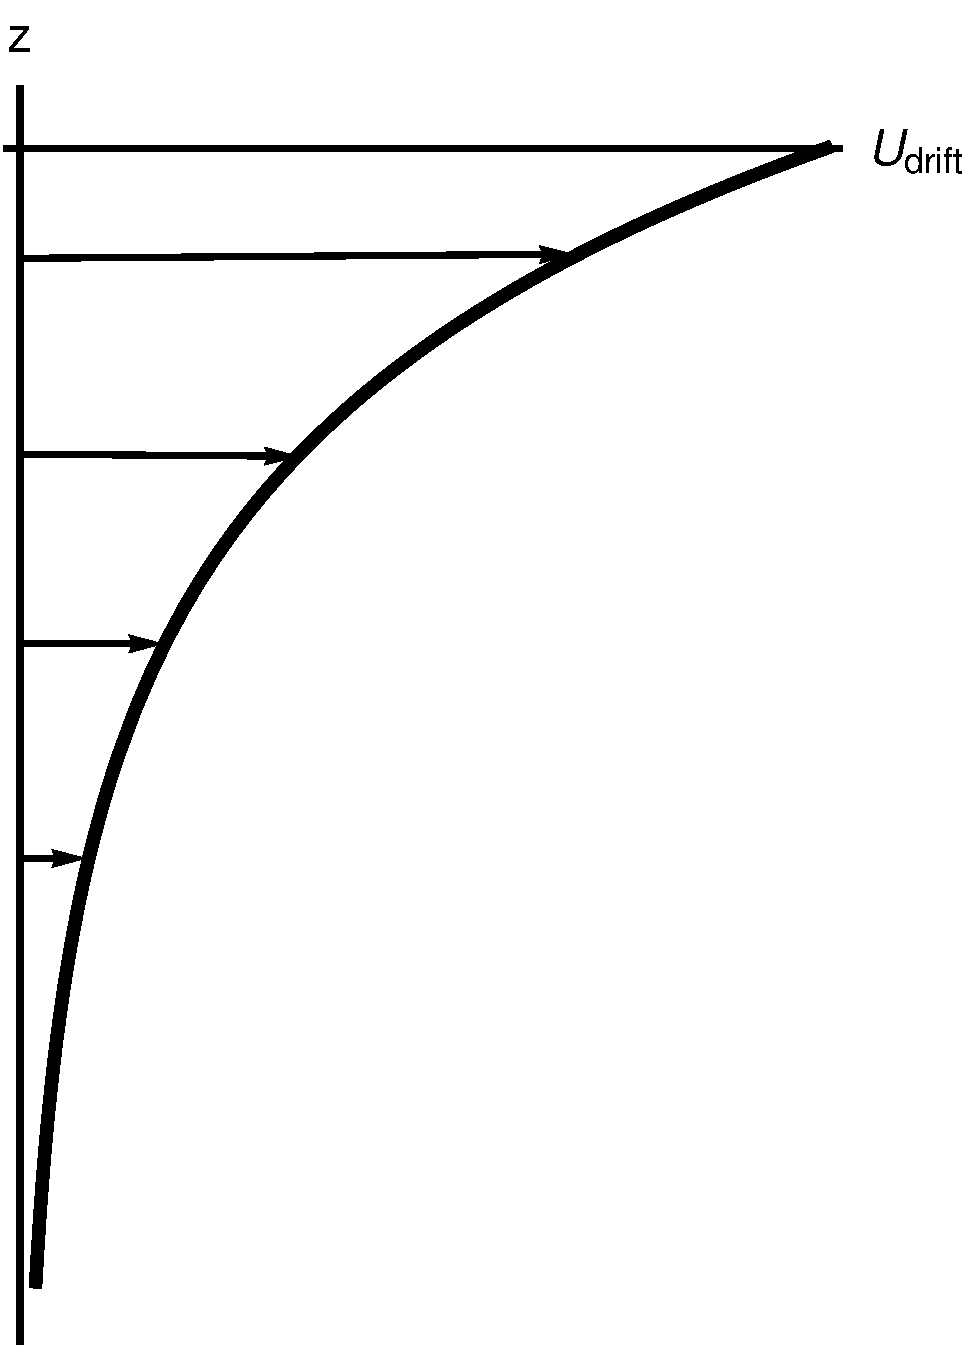
\includegraphics[scale=0.45]{Stokes_Drift_Profile.pdf}
\caption{Профиль классического дрейфа Стокса}\label{fig:Drift_Profile}
\end{figure}

Несмотря на давнюю историю, это явление активно изучается до сих пор и находит применение в различных приложениях \parencite{herreman2011stokes, feng2010ocean, christensen2009drift, rohrs2014wave, isobe2014selective}. 

Отдельный интерес для исследователей представляет волновое движение на границе раздела двух сред. В частности, если среды участвуют в относительном горизонтальном сдвиговом движении, то могут возникнуть условия для реализации неустойчивости Кельвина--Гельмгольца. Классическая постановка задачи возникает в системе двух идеальных полубесконечных несжимаемых жидкостей, в которой менее плотная жидкость с плотностью $ \rho ' $ движется с постоянной горизонтальной скоростью $ U_{0} $ относительно покоящейся жидкости с плотностью $ \rho $. Поле тяжести характеризуется ускорением свободного падения $ \mathbf{g} $, а поверхностное натяжение границы раздела --- коэффициентом поверхностного натяжения $ \gamma $. При достижении скоростью относительного сдвига некоторого критического значения $ U_{cr} $, величина которого определяется из дисперсионного уравнения
\begin{equation}
\omega=\dfrac{k \rho ' U_{0} \pm \sqrt{k g \left( \rho^{2} - \rho'^{2}\right) + k^{3} \gamma \left( \rho+ \rho' \right) - k^{2} \rho \rho' U_{0}^{2}}}{\rho+\rho'}
\label{DispUrKH}
\end{equation}
\noindent
амплитуда сколь угодно малых возмущений экспоненциально растет и на границе раздела образуются характерные вихри. При исследовании неустойчивости Кельвина--Гельмгольца обычно внимание уделяется эволюции границы раздела \parencite{Faber}, \parencite{Drazin}.

Еще одним очень интересным аспектом механики сплошных сред является описание траекторий движения индивидуальных частиц, составляющих жидкую среду при распространении волнового движения по ее поверхности. Исследование этого вопроса началось с работ \parencite{longuet1969transport}, в которой он обратил внимание на то, что период волнового движения (Эйлеров период) и период вращения жидкой частицы вокруг среднего положения (Лагранжев период) не совпадают и привел теорию для расчета этих периодов. В дальнейшем было математически показано, что траектория жидкой частицы должна быть незамкнута \parencite{henry2007particle}, \parencite{henry2007particle2}. Также были предложены численные методы для расчета траектории движения индивидуальных жидких частиц \parencite{chang2007particle}, \parencite{chang2009particle}.

Исторически сложилось, что все три выше перечисленных аспекта изучаются независимо друг от друга и, как правило, разными исследователями. Причем для описания дрейфовых движений обычно используется описание Лагранжа, а для описания траекторий и неустойчивости Кельвина--Гельмгольца задачу формулируют и решают в описании Эйлера. В настоящей главе предлагается аналитический асимптотический метод, в котором рассматриваются совместно три этих явления при помощи специально разработанной процедуры перехода между описанием Эйлера и Лагранжа.

\section{Формулировка задачи}\label{sec:ProcSnos}

Рассмотрим две идеальные полубесконечные несжимаемые несмешивающиеся жидкости в декартовой системе координат $ Oxyz $, в которой ось $ Oz $ направлена вертикально вверх против направления действия сил тяжести $ \mathbf{g} $. Нижняя жидкость с плотностью $ \rho $ занимает полупространство $ z<0 $, а верхняя менее плотная жидкость с плотностью $ \rho' < \rho $ занимает полупространство $ z>0 $ и движется поступательно с постоянной скоростью $ U_{0} $ в положительном направлении оси $ Ox $. Считается, что вдоль границы раздела, характеризуемой коэффициентом поверхностного натяжения $ \gamma $, в том же направлении распространяется периодическое волновое возмущение $ z=\xi \left(x, t\right) $ с длиной волны $ \lambda $. Движение жидкостей будем считать потенциальным и для простоты будем полагать его независящим от горизонтальной координаты $ y $. Задача решается в приближении волн малой амплитуды ($ \zeta \ll \lambda $). 
 
Существует два варианта описания поля скоростей в жидкости. Можно определять скорость жидких частичек в определенных (фиксированных) точках пространства и смотреть, как она изменяется с течением времени – это так называемое Эйлерово описание поля скоростей. Этот метод традиционно используется при описании задач механики жидкостей и он кажется более привычным, но у этого метода есть ряд недостатков. Основной причиной появления другого способа описания поля скоростей является то, что в этом случае невозможно проследить за траекторией и изменением скорости отдельной жидкой частички с течением времени. Действительно, зная скорость жидкой частички $ \mathbf{V}=\mathbf{V}\left( \mathbf{r}, t \right) $, неизвестно, в какой точке пространства она окажется в момент времени $ t+\Delta t $, если в момент времени $ t $ находилась в точке с радиус-вектором $ \mathbf{r} $. И даже несмотря на то, что известна скорость каждой частички жидкости в новый момент времени, невозможно узнать, где находится та частичка, за которой мы следили из-за того, что в Эйлеровом описании частички жидкости нельзя каким либо образом «пометить». Эта проблема решается при представлении поля скоростей в форме Лагранжа. Если в начальный момент времени $ t=t_{0} $ зафиксировать положение в пространстве и скорость индивидуальных жидких частичек и с течением времени следить за их изменениями, то мы сможем определить поле скоростей, «привязанное» не к позиции в пространстве, а к жидким частичкам. Скорость $ \mathbf{V}_{L}=\mathbf{V}_{L} \left( \mathbf{r}, t\right) $ определяет скорость жидкой частички, которая в начальный момент времени $ t=t_{0}=0 $ находилась в точке пространства с радиус вектором $ \mathbf{r} $. Поэтому кажется логичным формулировать и решать задачу в описании Лагранжа. Однако, в переменных Лагранжа возникают проблемы с корректной записью граничных условий на границе раздела двух идеальных жидкостей. Сказанное можно пояснить на примере условия равенства гидродинамических давлений в нижней ($ p_{L} \left( \mathbf{r}_{0}, t \right) $) и в верхней ($ p_{L}' \left( \mathbf{r}_{0}, t \right) $) жидкостях на границе раздела. Представим себе две жидкие частички, которые в начальный момент времени находились на границе раздела с разных ее сторон. Через некоторое произвольное время $ t $ в общем случае частицы идеальных жидкостей могут осуществить различный горизонтальный сдвиг и оказаться в разных точках границы раздела. В связи с этим запись условия баланса гидродинамических давлений в виде $ p_{L} \left( \mathbf{r}_{0}, t \right) =  p_{L}' \left( \mathbf{r}_{0}, t \right)  $ выглядит некорректной. 

Таким образом, записывать математическую формулировку задачи и проводить решение логичнее в описании Эйлера, в котором все переменные описывают свойства жидкости в определенной точке пространства с радиус-вектором $ \mathbf{r} $ в момент времени $ t $. При этом через эту точку пространства могут проходить различные жидкие частицы и для определения их скорости необходимо будет осуществлять дополнительные математические операции.

В переменных Эйлера математическая формулировка задачи по определению гидродинамических потенциалов нижней $ \varphi $ и верхней $ \varphi ' $ жидкостей имеет вид: 
\begin{gather}
\begin{gathered}
z>\xi :\mspace{190mu}  \Delta \varphi'=0;\mspace{190mu} \\
 P'=p_{0}-\rho' g z-\rho' \partial_{t}\varphi' - \left( \rho' /2 \right) \left[ \left( \partial_{x} \varphi' +U_{0}\right)^{2} +\left( \partial_{z} \varphi' \right)^{2}\right] ;\label{Euler}
\end{gathered}
\\
\begin{gathered}
z=\xi : \qquad \partial_{t}\xi + \partial_{x} \xi \partial_{x}\varphi =\partial_{z} \varphi ;\qquad  \partial_{t}\xi + \left( \partial_{x}\varphi' +U_{0} \right)  \partial_{x} \xi =\partial_{z} \varphi' ;
\\
\qquad \qquad \qquad P-P'=-\gamma \partial_{xx}\xi \left( 1+\left( \partial_{x} \xi\right)^{2} \right)^{-3/2} ;
\end{gathered}\label{GrUsl}
\\
\begin{gathered}
z<\xi : \mspace{190mu} \Delta \varphi=0;\mspace{190mu}\\
P=p_{0}-\rho g z-\rho \partial_{t}\varphi - \left( \rho /2 \right) \left[ \left( \partial_{x} \varphi\right)^{2} +\left( \partial_{z} \varphi \right)^{2}\right] ;\label{Euler2}
\end{gathered}
\\
z\rightarrow \infty : \qquad \qquad \nabla \varphi' \rightarrow 0 ;\qquad \qquad z\rightarrow -\infty :\qquad \qquad \nabla \varphi \rightarrow 0.\label{BeskUsl}
\end{gather}
 Здесь $ P $ и $ P' $~--- гидродинамическое давление в нижней и верхней средах соответственно, а $ p_{0} $~--- постоянная внешняя составляющая играющая роль атмосферного давления. 
Будем решать задачу в приближении волн малой амплитуды методом разложения по малому параметру $ \varepsilon = \zeta k $, показывающему отношение амплитуды волны $ \zeta $ к ее длине $ \lambda=2\pi /k $. Дрейф Стокса – явление второго порядка малости по амплитуде волны, поэтому разложение искомых величин будем находить с точностью до второго порядка:

\begin{equation}
\begin{pmatrix}
\xi
\\
\varphi
\\
\varphi'
\end{pmatrix} = \begin{pmatrix}
\xi_{1}
\\
\varphi_{1}
\\
\varphi'_{1}
\end{pmatrix} + \begin{pmatrix}
\xi_{2}
\\
\varphi_{2}
\\
\varphi'_{2}
\end{pmatrix}+ O\left( \varepsilon^{3}\right). 
\label{Razl}
\end{equation}
 
 Здесь $ O $~--- символ Ландау, характеризующий порядок остаточных слагаемых по $ \varepsilon $.

Наряду с разложением (\ref{Razl}), применялась известная процедура снесения граничных условий (\ref{GrUsl}) на невозмущенную поверхность $ z=0 $, обоснование которой представлено в \parencite{joseph1973domain}, а примеры использования можно посмотреть в \parencite{vakbib4}, \parencite{Levich}, \parencite{mcgoldrick1972rippling}, \parencite{nayfeh1971method}. Так, для значений горизонтальной скорости течения 
$ \partial_{z} \varphi $ со стороны нижней области  снесение с поверхности $ z=\xi $ на уровень $z=0$ осуществляется посредством следующих выкладок:
\begin{eqnarray*}
\left( \dfrac{\partial \varphi}{\partial z}\right)_{z=\xi}=\left( \dfrac{\partial \varphi}{\partial z}\right)_{z=0} + \xi \left( \dfrac{\partial^{2} \varphi}{\partial z^{2}}\right)_{z=0} + \dfrac{1}{2} \xi^{2} \left( \dfrac{\partial^{3} \varphi}{\partial z^{3}}\right)_{z=0}+ \ldots = 
\\
=\left( \dfrac{\partial  \left( \varphi_{1}+\varphi_{2}\right)}{\partial z}\right)_{z=0} +  \left( \xi_{1}+\xi_{2}\right)  \left( \dfrac{\partial^{2} \left( \varphi_{1}+\varphi_{2}\right) }{\partial z^{2}}\right)_{z=0}+ \ldots = 
\\
=\left( \dfrac{\partial \varphi_{1}}{\partial z}\right)_{z=0} + \left( \dfrac{\partial \varphi_{2}}{\partial z}\right)_{z=0} + \xi_{1} \left( \dfrac{\partial^{2} \varphi_{1}}{\partial z^{2}}\right)_{z=0} + \ldots
\label{Poyasnenie}
\end{eqnarray*}
Видно, что значение, которое величина  принимает на искривленной поверхности $z=\xi(x,t)$, оказалось  с необходимой степенью точности выраженным через через значение этой же величины и значения ее производных  на уровне $z=0$. 
С помощью~\eqref{Razl} и процедуры снесения граничных условий на невозмущенный уровень, несложно перейти от~\eqref{Euler}~---~\eqref{BeskUsl} к задачам первого и второго порядков малости.  

Математическая формулировка  задачи первого по $ \varepsilon $ порядка малости имеет вид:
\begin{align}
&z>0 : \qquad \qquad \Delta \varphi_{1}'=0; \qquad \qquad \qquad  z<0 : \qquad \qquad \Delta \varphi_{1}=0; \label{Eul1}
\\
&z=0 : \qquad \partial_{t}\xi_{1} -\partial_{z} \varphi_{1}=0 ; \qquad  \partial_{t}\xi_{1} + U_{0}  \partial_{x} \xi_{1} -\partial_{z} \varphi'_{1}=0 ;
\\
&\qquad \qquad g \xi_{1}\left( \rho' -\rho \right)-\rho \partial_{t} \varphi_{1}+\rho' \partial_{t} \varphi'_{1}+\rho' U_{0} \partial_{x} \varphi'_{1}+\gamma \partial_{xx}\xi_{1}=0 ;
\\
&z\rightarrow \infty : \qquad \qquad \nabla \varphi'_{1} \rightarrow 0 ;\qquad \qquad z\rightarrow -\infty :\qquad \qquad \nabla \varphi_{1} \rightarrow 0.\label{Besk1}
\end{align}

Задача второго по $ \varepsilon $ порядка малости описывается соотношениям:
\begin{equation}
z>0 : \qquad \qquad \Delta \varphi_{2}'=0; \qquad \qquad \qquad  z<0 : \qquad \qquad \Delta \varphi_{2}=0;\label{Eul2}
\end{equation} 
\begin{gather}
\begin{gathered}
z=0 : \mspace{108mu} \partial_{t}\xi_{2} -\partial_{z} \varphi_{2}=\xi_{1} \partial_{zz}\varphi_{1}-\partial_{x}\varphi_{1}\xi_{1};\mspace{108mu}
\\ 
 \partial_{t}\xi_{2} + U_{0}  \partial_{x} \xi_{2} -\partial_{z} \varphi'_{2}=\xi_{1} \partial_{zz} \varphi'_{1}-\partial_{xx}\varphi'_{1} \partial_{xx}\xi_{1} ;
\\
 g \xi_{2}\left( \rho' -\rho \right)-\rho \partial_{t} \varphi_{2}+\rho' \partial_{t} \varphi'_{2}+\rho' U_{0} \partial_{x} \varphi'_{2}+\gamma \partial_{xx}\xi_{2}= \\
 =\rho \xi_{1} \partial_{zt} \varphi_{1}+\dfrac{\rho}{2}\left( \left( \partial_{x}\varphi_{1}\right)^{2} +\left( \partial_{z}\varphi_{1}\right)^{2}\right)- \rho' \xi_{1} \partial_{zt} \varphi'_{1} - \\
 -\dfrac{\rho'}{2} \left( \left( \partial_{x}\varphi'_{1}\right)^{2} +\left( \partial_{z}\varphi'_{1}\right)^{2}+2U_{0} \xi_{1} \partial_{xx} \varphi'_{1}\right); \label{GU2}
\end{gathered}
\end{gather}
\begin{equation}
z\rightarrow \infty : \qquad \qquad \nabla \varphi'_{2} \rightarrow 0 ;\qquad \qquad z\rightarrow -\infty :\qquad \qquad \nabla \varphi_{2} \rightarrow 0.\label{Besk2}
\end{equation}

Последовательное решение сначала~\eqref{Eul1}~---~\eqref{Besk1},
затем ~\eqref{Eul2}~---~\eqref{Besk2}  приводит к аналитическим выражениям, позволяющим описать эйлерово
поле скоростей во втором приближении по $\varepsilon $. При этом начальные условия заменяются условием поиска решения в наиболее простом (в аналитическом плане) виде описывающем периодическую бегущую волну длиной $ \lambda $.

\section{Свойства решения} \label{sec:ch2/sec3}

Решение задачи первого порядка малости~\eqref{Eul1}~---~\eqref{Besk1} в виде простейшей бегущей волны записывается следующим образом:
\begin{equation}
\begin{pmatrix}
\xi_{1}
\\
\varphi_{1}
\\
\varphi'_{1}
\end{pmatrix}= \dfrac{1}{2}\zeta \exp \left( i\omega t-i k x\right) \begin{pmatrix}
1
\\
-i\left(\omega -k U_{0}\right)/k
\\
i \omega/k
\end{pmatrix}+ C.C. 
\label{Resh1}
\end{equation}

Здесь символ $ C.C. $ определяет комплексно сопряженные слагаемые, $ i $~--- мнимая единица, а круговая частота $ \omega $ связана с волновым числом и другими параметрами задачи посредством дисперсионного уравнения~\eqref{DispUrKH}.

Анализ дисперсионного уравнения показывает, что при движении верхней жидкости со скоростью меньшей некоторого критического значения \[U_{0}\leq U_{cr}\left( k \right)=\sqrt{\dfrac{k^{2} \gamma \left( \rho+\rho' \right) +g \left( \rho^{2}-\rho'^{2} \right)}{k \rho \rho'}}\] круговая частота  принимает действительные значения. Следовательно, все компоненты решения задачи будут периодическими функциями. В случае когда $ U_{0}>U_{cr}\left( k \right) $ частота $ \omega $ принимает комплексные значения и в решении появляется множитель $ \propto\exp \left( \pm Im\left( \omega t \right) \right) $. Таким образом происходит распространение волн с экспоненциально нарастающей амплитудой. Такое движение связывают с начальными этапами развития неустойчивости Кельвина--Гельмгольца. На рисунке~\ref{fig:K_H_Neutral} показана кривая нейтральной устойчивости в области параметров величины тангенциального разрыва скоростей на границе раздела и волнового числа бегущей по этой границе синусоидальной волны $ \left( U_{0}, k \right) $. Кривая построена в безразмерных переменных, в которых $ \rho=g=\gamma=1 $, стандартных для этого типа задач гидродинамики. Область (1) ниже этой кривой соответствует устойчивому волновому движению, а область (2) выше кривой --- развитию неустойчивости Кельвина--Гельмгольца. Из рисунка~\ref{fig:K_H_Neutral} видно, что существует такое волновое число \[k_{cr}=\sqrt{\dfrac{g \left( \rho - \rho' \right)}{\gamma}},\] которое наиболее восприимчиво к возникновению неустойчивости Кельвина--Гельмгольца. Соответствующая ему критическая скорость реализации неустойчивости Кельвина--Гельмгольца
\begin{equation}
U_{cr}=\sqrt{\dfrac{2 \left( \rho + \rho' \right) \sqrt{\gamma g \left( \rho - \rho' \right)}}{\rho \rho'}}.
\label{Ucrit}
\end{equation}

\begin{figure}[ht]
\centering
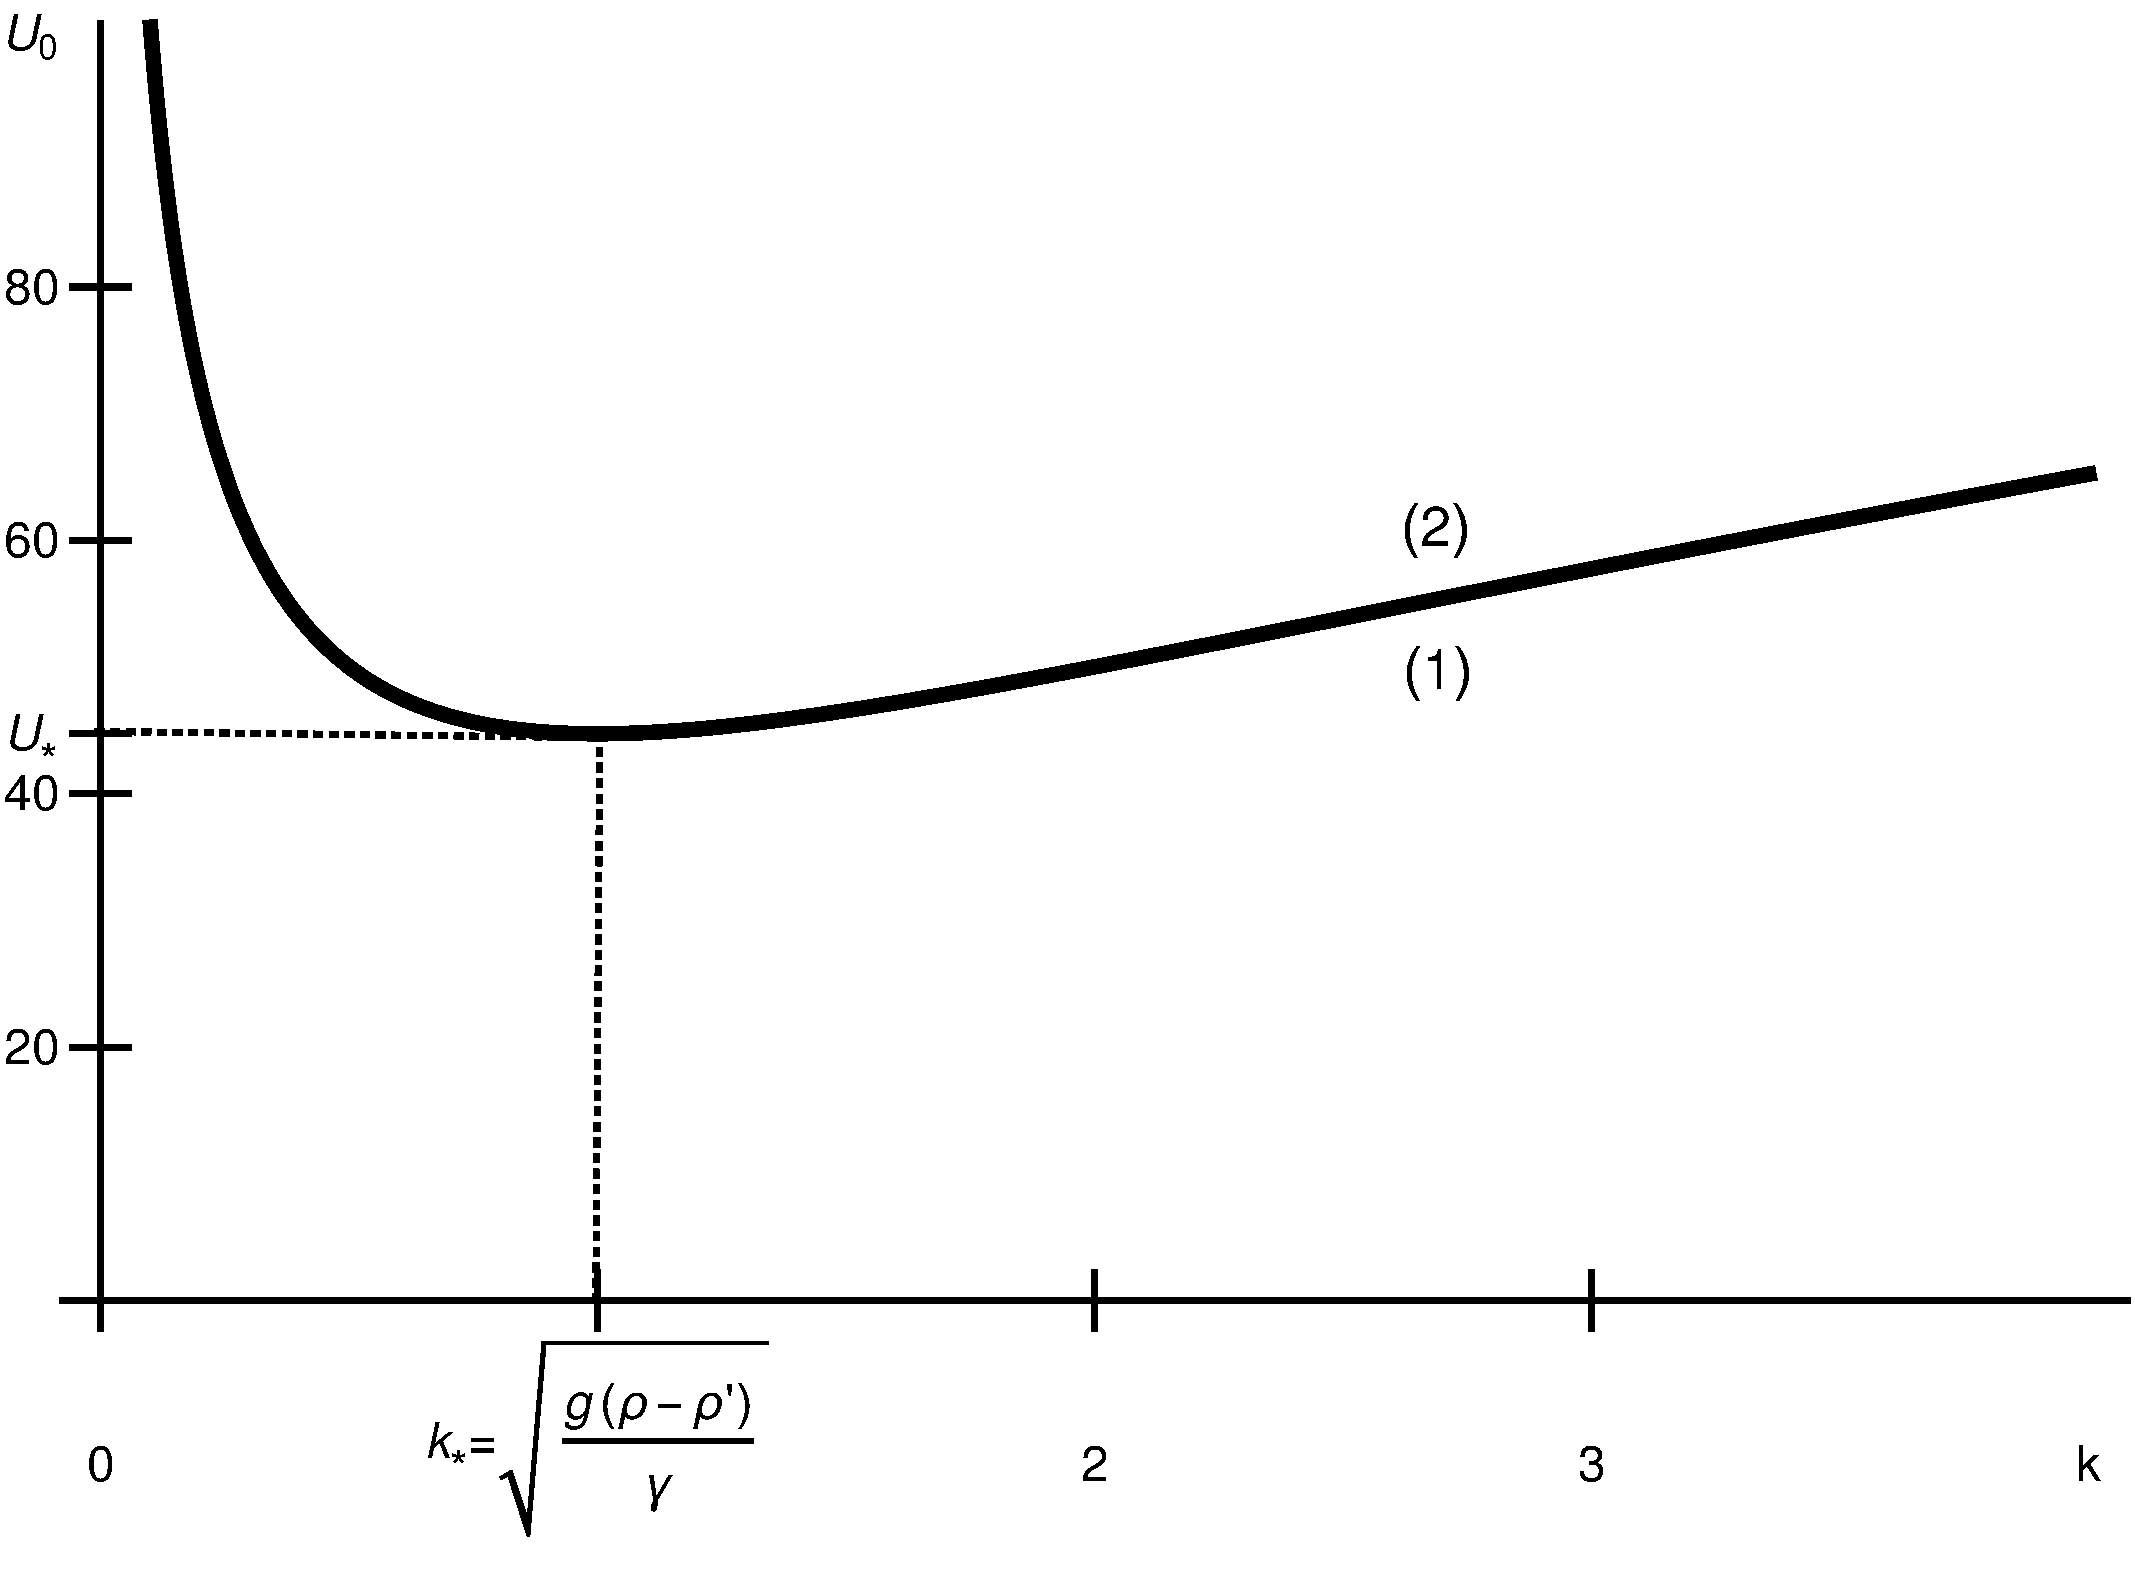
\includegraphics[scale=0.4]{K_H_Neutral.pdf}
\caption{Кривая нейтральной устойчивости неустойчивости Кельвина--Гельмгольца в безразмерных переменных $ \rho=g=\gamma=1 $}\label{fig:K_H_Neutral}
\end{figure}

Из решения задачи для гидродинамических потенциалов несложно получить выражения для горизонтальных и вертикальных составляющих скоростей в линейном приближении по амплитуде волнового движения. В нижней жидкости горизонтальная $ u_{1} $ и вертикальная $ v_{1} $ компоненты выражаются следующим образом:
\begin{equation}
u_{1}=\dfrac{1}{2}\zeta \omega \exp \left( i \left( \omega t -k x\right) \right) \exp \left( k z \right) +C.C.
\label{u1}
\end{equation}
\begin{equation}
v_{1}=-\dfrac{i}{2}\zeta \omega \exp \left( i \left( \omega t -k x\right) \right) \exp \left( k z \right) +C.C.
\label{v1}
\end{equation}

В верхней жидкости горизонтальная  $ u'_{1} $ и вертикальная $ v'_{1} $ составляющая имеют вид:
\begin{equation}
u'_{1}=U_{0}-\dfrac{1}{2}\zeta \left( \omega - k U_{0}\right) \exp \left( i \left( \omega t -k x\right) \right) \exp \left( -k z \right) +C.C.
\label{u1'}
\end{equation}
\begin{equation}
v'_{1}=\dfrac{i}{2}\zeta \left( \omega - k U_{0}\right)  \exp \left( i \left( \omega t -k x\right) \right) \exp \left( -k z \right) +C.C.
\label{v1'}
\end{equation}

Подставляя решение~\eqref{Resh1} в правые части граничных условий задачи второго порядка малости~\eqref{GU2} можно заметить, что неоднородности являются периодическими функциями $ \Pi \left(2 \left( \omega t-k x\right) \right) $, пропорциональные $ \propto~\!\!\!\!\sin \left(2 \left( \omega t-k x\right) \right) $ или $ \propto~\!\!\!\!\cos \left(2 \left( \omega t-k x\right) \right) $. Следовательно, решение задачи второго порядка малости содержит в себе в качестве множителя функцию вида $ \Pi \left(2 \left( \omega t-k x\right) \right) $. 

\section{Принцип перехода к переменным Лагранжа}\label{sec:Pereh}

Для определения дрейфовой скорости и для расчета движения индивидуальных жидких частиц используется описание поля скоростей в форме Лагранжа $ \mathbf{V}_{L}\left( \mathbf{r}, t\right) = \mathbf{e}_{x} u_{L}+ \mathbf{e}_{z} v_{L}$. Существует процедура перехода от описания поля скоростей в Эйлеровой форме к описанию поля скоростей в Лагранжевой форме. Приведем вывод асимптотической формулы перехода в предположении малости волнового возмущения. Очевидно, что в нулевой момент времени $ t=t_{0}=0 $ скорость жидкой частички в форме Эйлера и в форме Лагранжа совпадают: $ \mathbf{V}\left( \mathbf{r}, t\right)=\mathbf{V}_{L}\left( \mathbf{r}, t\right)$. Рассмотрим перемещение выделенной жидкой частички, через отрезок времени $ \tau $ (причем время $ \tau $ не будем считать малым) она окажется в точке с радиус-вектором $ \mathbf{r}+\delta \mathbf{r} $. В приближении волн малой амплитуды можно считать, что перемещение жидкой частички $ \delta \mathbf{r} $ за конечный промежуток времени мало по сравнению с амплитудой волнового движения. Такая ситуация в природе встречается например при распространении капиллярно-гравитационных волн малой амплитуды в струях, по поверхности мирового океана, при малых колебаниях капли, и именно такое движение мы и будем рассматривать. На рисунке~\ref{fig:Pereh} демонстрируется смещение жидкой частички, участвующей в таком движении, при этом за конечное время смещение составляет величину меньшую чем амплитуда волнового возмущения. 
\begin{figure}[ht]
\centering
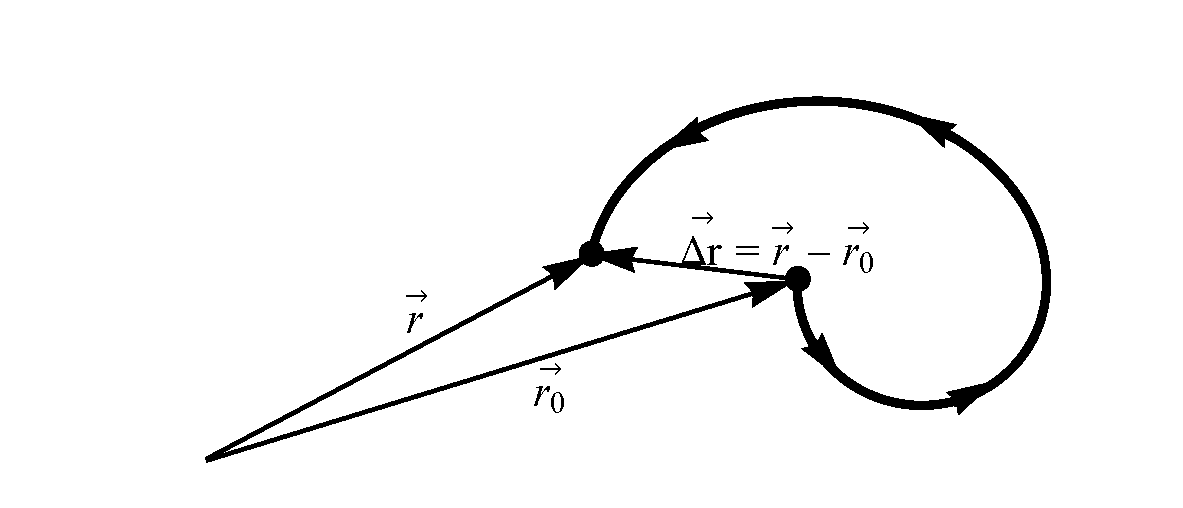
\includegraphics[scale=0.5]{Pereh.pdf}
\caption{Смещение индивидуальной жидкой частички за конечное время~$ t $}\label{fig:Pereh}
\end{figure}
В новом положении скорость в форме Лагранжа $ \mathbf{V}_{L}\left( \mathbf{r}, \tau\right) $ равна скорости в форме Эйлера $ \mathbf{V}\left( \mathbf{r}+\delta \mathbf{r}, \tau \right) $, значит можно выразить разность: \[ \mathbf{V}_{L}\left( \mathbf{r}, \tau\right)-  \mathbf{V}\left( \mathbf{r}, \tau \right) = \mathbf{V}\left( \mathbf{r}+\delta \mathbf{r}, \tau \right) - \mathbf{V}\left( \mathbf{r}, \tau \right). \] Разложим правую часть этого выражения в ряд Маклорена и в силу малости перемещения  можем аппроксимировать ее только главными членами ряда: 
\begin{equation}
\mathbf{V}_{L}\left( \mathbf{r}, \tau\right)-  \mathbf{V}\left( \mathbf{r}, \tau \right) = \left( \delta \mathbf{r} \cdot \nabla \right) \mathbf{V}\left( \mathbf{r}, \tau \right) + \Upsilon
\label{Macloren}
\end{equation}
Здесь $ \Upsilon $~--- остаточный член, который по порядку не превосходит произведений квадрата вектора $ \delta \mathbf{r} $ на вторые производные по координатам компонент вектора скорости $ \mathbf{V}\left( \mathbf{r}, \tau \right) $. 

Лагранжева скорость определяет скорость выделенной частички жидкости, потому ее перемещение  $ \delta \mathbf{r} $ за время $ \tau $ можно определить простым интегрированием:
\begin{equation}
 \delta \mathbf{r} = \int_{0}^{\tau} \mathbf{V}_{L}\left( \mathbf{r},t \right)d t
 \label{Int}
\end{equation}
	 
Подставляя интеграл~\eqref{Int} в~\eqref{Macloren} получим выражение для расчета скорости Лагранжа:
\begin{equation}
\mathbf{V}_{L}\left( \mathbf{r}, \tau\right) = \mathbf{V}\left( \mathbf{r}, \tau \right) + \left( \left( \int_{0}^{\tau} \mathbf{V}_{L}\left( \mathbf{r},t \right)d t\right) \cdot \nabla \right) \mathbf{V}\left( \mathbf{r}, \tau \right) + \Upsilon
\label{MaclorenInt}
\end{equation}

Если вместо подынтегрального выражения в~\eqref{MaclorenInt} поставить всю правую часть~\eqref{MaclorenInt}, предварительно заменив в ней $ t $ на $ t_{1} $, а $ \tau $ на $ t $, то соотношение~\eqref{MaclorenInt} преобразуется к виду:
\begin{multline}
\mathbf{V}_{L}\left( \mathbf{r}, \tau \right) = \mathbf{V}\left( \mathbf{r}, \tau \right) +\\
+ \left\lbrace  \left[ \int_{0}^{\tau}\left( \mathbf{V}\left( \mathbf{r}, \tau \right) +\left( \left( \int_{0}^{t}\mathbf{V}\left( \mathbf{r}, t_{1} \right)d t_{1}\right) \cdot \nabla \right)\times \right. \right. \right. \\
\left. \left. \left. \times \mathbf{V}\left( \mathbf{r}, t \right) + \Upsilon \right) d t \right] \cdot \nabla \right\rbrace  \mathbf{V}\left( \mathbf{r}, \tau \right) +\Upsilon
\label{Asimptot}
\end{multline}
	 
Поскольку скорость выделенной индивидуальной частички жидкости  мала по сравнению с фазовой скоростью волн, в асимптотической формуле~\eqref{Asimptot} правомерно оставить только главный член представления:
\begin{equation}
\mathbf{V}_{L}\left( \mathbf{r}, \tau\right) = \mathbf{V}\left( \mathbf{r}, \tau \right) + \left( \left( \int_{0}^{\tau} \mathbf{V}\left( \mathbf{r},t \right)d t\right) \cdot \nabla_{0} \right) \mathbf{V}\left( \mathbf{r}, \tau \right) 
\label{Pereh}
\end{equation}

Нижний индекс «0» при операторе $ \nabla $ означает, что частные производные вычисляются в положении, в котором частичка находилась в начальный момент времени. Таким образом, приходим к асимптотическому выражению лагранжевой скорости индивидуальной жидкой частички через эйлерову скорость. Выражение~\eqref{Pereh} по известному полю скоростей в эйлеровом представлении позволяет получить скорость жидкой частички, которая в нулевой момент времени $ t=t_{0}=0 $ находилась в точке пространства с радиус-вектором $ \mathbf{r} $. Простое интегрирование по времени этого выражения позволит нам построить реальную траекторию движения индивидуальной жидкой частички. Но здесь важно обратить внимание на границы применимости формулы. Во-первых, она применима только для определения лагранжевой скорости не больше чем второго порядка малости по амплитуде волны, поскольку мы при расчете использовали приближение эйлеровой скорости второго порядка малости. Во-вторых, изначально накладывалось ограничение на перемещение индивидуальной жидкой частички $ \delta \mathbf{r} $ --- оно должно удовлетворять условию малости по сравнению с амплитудой волны. Поэтому формула неприменима в условиях больших сдвигов жидких частичек. В-третьих, использовать формулу перехода~\eqref{Pereh} возможно лишь для волн малой по сравнению с длиной амплитуды. Все эти ограничения важно учитывать при расчетах в различных приложениях.

\section{Применение принципа расчета скорости жидких частиц к двухслойной системе}

Применяя~\eqref{Pereh} к полю скоростей~\eqref{u1}~---~\eqref{v1} в первом по $ \varepsilon $ приближении получим, что скорости нижней жидкости в представлении Лагранжа описываются при помощи выражений:
\begin{equation}
u_{L1}=\dfrac{1}{2}\zeta \omega \exp \left( i\omega t-i k x_{0} \right) \exp \left( k z_{0} \right) +C.C.
\label{ul1}
\end{equation}
\begin{equation}
v_{L1}=-\dfrac{i}{2}\zeta \omega \exp \left( i\omega t-i k x_{0} \right) \exp \left( k z_{0} \right) +C.C.
\label{vl1}
\end{equation}

Здесь $ x_{0} $ и $ z_{0} $ играют роль координаты начального положения индивидуальной жидкой частицы. Таким образом, в первом приближении переход от описания Эйлера к описанию Лагранжа сводится к изменению статуса координат. Такое формальное совпадение скоростей в описании Эйлера и Лагранжа в первом приближении давно известно и часто используется для описания движения материальных частиц по круговым траекториям \parencite{Landau}, \parencite{Levich}, \parencite{Sivukhin}. 
Так как в неподвижной системе координат $ Oxyz $ жидкие частицы верхней жидкости помимо волнового движения участвуют в сдвиговом течении со скоростью $ U_{0} $ и за время $ \tau $ смещаются на немалое расстояние $ U_{0} \tau $ по горизонтали, то в силу границ применимости формулы перехода~\eqref{Pereh} невозможно ее простое аналогичное применение к полю скоростей верхней жидкости~\eqref{u1'}~---~\eqref{v1'}. Для корректного применения формулы перехода к полю скоростей~\eqref{u1'}~---~\eqref{v1'} необходимо перейти в систему координат $ O^{*}x^{*}y^{*}z^{*} $, движущуюся синхронно с верхней жидкостью. Если в начальный момент времени $ t=t_{0}=0 $ системы координат $ Oxyz $ и $ O^{*}x^{*}y^{*}z^{*} $ совпадают, то новые координаты выражаются через старые следующим образом:
\begin{equation*}
\begin{pmatrix}
x^{*}
\\
y^{*}
\\
z^{*}
\end{pmatrix}= \begin{pmatrix}
x-U_{0}t
\\
y
\\
z
\end{pmatrix} 
\end{equation*}

При этом частота волнового движения изменяется из-за эффекта Доплера соответствующим образом:
\begin{equation}
\omega t-k x=\omega t -k \left( x^{*}+U_{0} t \right) = \Omega t -k x^{*}
\label{omega}
\end{equation}
\begin{equation*}
\Omega = \omega - k U_{0}
\end{equation*}

Тогда периодические функции, содержащие в качестве аргумента круговую частоту преобразуются:
\begin{equation*}
\cos \left( \omega t-k x \right) \rightarrow \cos \left( \Omega t -k x^{*} \right)
\end{equation*}
\begin{equation*}
\sin \left( \omega t-k x \right) \rightarrow \sin \left( \Omega t -k x^{*} \right)
\end{equation*}

В новой системе координат Эйлерово поле скоростей в первом приближении по амплитуде волны выглядит следующим образом:
\begin{equation}
u'^{*}_{1}=-\dfrac{1}{2}\zeta  \Omega  \exp \left( i \left( \Omega t -k x^{*}\right) \right) \exp \left( -k z^{*} \right) +C.C.
\label{u1'*}
\end{equation}
\begin{equation}
v'^{*}_{1}=\dfrac{i}{2}\zeta  \Omega \exp \left( i \left( \Omega t -k x^{*}\right) \right) \exp \left( -k z^{*} \right) +C.C.
\label{v1'*}
\end{equation}

В движущейся системе координат применение формулы перехода~\eqref{Pereh} к полю скоростей~\eqref{u1'*}~---~\eqref{v1'*} правомерно и скорость в описании Лагранжа в системе координат $ O^{*}x^{*}y^{*}z^{*} $ имеет вид:
\begin{equation*}
u'^{*}_{L1}=-\dfrac{1}{2}\zeta \Omega \exp \left( i\Omega t-i k x^{*}_{0} \right) \exp \left(-k z^{*}_{0} \right) +C.C.
\end{equation*}
\begin{equation*}
v'^{*}_{L1}=\dfrac{i}{2}\zeta \Omega \exp \left( i\Omega t-i k x^{*}_{0} \right) \exp \left(- k z^{*}_{0} \right) +C.C.
\end{equation*}

Совершая обратный переход в неподвижную систему координат  получим:
\begin{equation}
u'_{L1}=U_{0}-\dfrac{1}{2}\zeta \Omega \exp \left( i\Omega t-i k x_{0} \right) \exp \left(-k z_{0} \right) +C.C.
\label{ul1'}
\end{equation}
\begin{equation}
v'_{L1}=\dfrac{i}{2}\zeta \Omega \exp \left( i\Omega t-i k x_{0} \right) \exp \left(- k z_{0} \right) +C.C.
\label{vl1'}
\end{equation}	 	
	 	
Поскольку в начальный момент времени подвижная и неподвижная системы координат совпадают, то справедливы равенства $ x_{0}=x^{*}_{0} $ и $ z_{0}=z^{*}_{0} $. При обратном переходе не требуются преобразования частоты $ \Omega $, обратные преобразованиям~\eqref{omega}. В этом случае речь идет не о частоте волнового движения, а о частоте круговых движений выделенной жидкой частицы. Здесь уместна аналогия с частотой колебаний маятника: циклические движения индивидуальной материальной частицы представляют из себя своего рода часовой механизм, а в рамках классической механики период часового механизма не меняется в инерциальных системах отсчета, следовательно неизменной остается частота круговых движений жидких частиц $ \Omega $.

\subsection{Дрейфовые и циклические составляющие скорости}

Из формулы перехода~\eqref{Pereh} видно, что горизонтальная скорость выделенной жидкой частички с точностью до второго по $ \varepsilon $ порядка малости определяется выражением:
\begin{multline}
u_{L}\left( x_{0}, z_{0}, t\right) = u_{1}\left( x_{0}, z_{0}, t\right)+u_{2}\left( x_{0}, z_{0}, t\right)+\\
+ \left( \int_{0}^{t}u_{1}\left( x_{0}, z_{0}, t\right)d \tau \right)\left( \dfrac{\partial u_{1}\left( x, z, t\right)}{\partial x}\right)_{\substack{x=x_{0}\\z=z_{0}}}+\\
+\left( \int_{0}^{t}v_{1}\left( x_{0}, z_{0}, t\right)d \tau \right)\left( \dfrac{\partial u_{1}\left( x, z, t\right)}{\partial z}\right)_{\substack{x=x_{0}\\z=z_{0}}}
\label{ulDrift}
\end{multline}

Выделим из скорости движения материальной частицы слагаемые, отвечающие за дрейф (дрейфовые слагаемые) и слагаемые, отвечающие за круговые движения (циклические слагаемые). Заметим, что первое и второе слагаемое в~\eqref{ulDrift} описываются периодическими функциями (см. выражения~\eqref{u1}~---~\eqref{v1} и соображения в заключении раздела~\ref{sec:ch2/sec3}). Таким образом, эти слагаемые отвечают за циклические движения материальных частиц и не вносят вклад в дрейфовые движения. Третье и четвертое слагаемое в~\eqref{ulDrift} (интегральные слагаемые) при подстановке~\eqref{u1}~---~\eqref{v1} и вычислении помимо циклических слагаемых вида $ \Pi \left( 2 \omega t - 2 k x \right) $ включают в себя дрейфовую компоненту скорости:
\begin{equation}
U_{DS}=\zeta^{2} \omega k \exp \left(2 k z\right),
\label{UdriftNizh}
\end{equation}
аналогичную выражению, полученного для классического дрейфа Стокса~\eqref{DriftStokes}.

Расчет скорости горизонтального дрейфа жидких частиц верхней жидкости сопряжен с особенностями, изложенными в предыдущем пункте. Проделав все необходимые математические процедуры, несложно получить дрейфовую компоненту скорости верхней жидкости:
\begin{equation}
U'_{DS}=U_{0}+\zeta^{2} \Omega k \exp \left(-2 k z\right),
\label{UdriftVerh}
\end{equation}

Обратим внимание на факт, что через некоторый большой (по сравнению с периодом обращения индивидуальной жидкой частицы) промежуток времени жидкие частицы, увлекаемые даже малым дрейфом~\eqref{UdriftNizh}, сместятся на большое (по сравнению с длиной волны) расстояние. И тогда формула перехода~\eqref{Pereh} выходит за границы применимости. Таким образом, для корректного расчета дрейфа даже в нижней жидкости нужно переходить в систему отсчета, дрейфующую вместе с жидкими частицами. Осуществляя математические процедуры, описанные в предыдущем пункте можно найти усовершенствованную форму записи лагранжевых компонент скорости жидких частиц нижней жидкости:
\begin{equation}
u_{L1}=\dfrac{1}{2}\zeta \omega \exp \left( i\left( \left( \omega - k U_{DS} \right) t- k x_{0}\right) \right) \exp \left( k z_{0} \right) +C.C.
\label{ul1Mod}
\end{equation}
\begin{equation}
v_{L1}=-\dfrac{i}{2}\zeta \omega \exp \left( i\left( \left( \omega - k U_{DS} \right) t- k x_{0}\right) \right) \exp \left( k z_{0} \right) +C.C.
\label{vl1Mod}
\end{equation}

Из~\eqref{ul1Mod}~---~\eqref{vl1Mod} можно заметить, что период $ \tau=2\pi / \left( \omega - k U_{DS} \right) $ круговых движений индивидуальной жидкой частицы больше периода волнового движения границы раздела $ T=2\pi / \omega $. Этот факт играет важную роль в согласовании движения материальных частиц, находящихся на границе раздела жидких сред и участвующих в циклических и дрейфовых движениях с движениями этой границы. 

Рассмотрим это явление на примере одной жидкой частички, в начальный момент времени находящуюся во впадине волны, возмущающей границу раздела~\eqref{Resh1}. Через время $ \tau $ частичка оказывается снова в нижней части своей траектории. При этом она движется по траектории сначала поднимаясь, а потом снова опускаясь в следующую впадину волны. Так как период волнового движения $ T $ меньше периода обращения жидкой частицы $ \tau $, нижняя точка впадины, в которой окажется жидкая частица, будет иметь горизонтальную координату не $ x_{0} $, а $ x=x_{0}+U_{ph}\left( \tau -T\right) $, где $ U_{ph}=\omega/k $ – фазовая скорость волнового возмущения границы раздела~\eqref{Resh1}. Жидкая частичка за это время по горизонтали смещается в положительном направлении оси $ Ox $ на расстояние $ \Delta x = \omega \left( \tau -T\right)/k $. Скорость смещения жидкой частички в горизонтальном направлении определяется отношением $ \Delta x/\tau $. Подставив сюда значения периодов волнового движения и циклического движения индивидуальной жидкой частицы получим:
\begin{equation*}
\dfrac{\Delta x}{\tau}=\dfrac{\left( \tau -T\right) \omega}{k \tau}=\left( \dfrac{2 \pi}{\omega - k U_{DS} } - \dfrac{2 \pi}{\omega}\right)\dfrac{\omega \left( \omega - k U_{DS}\right)}{2 \pi k}=U_{DS}
\end{equation*}

Действительно получается, что, исходя из таких соображений траектория движения индивидуальной жидкой частицы оказывается согласованной с формой волнового возмущения границы раздела. Если же не брать в расчет разницу в периодах волнового возмущения и кругового движения жидкой частицы, то совершающая витки и дрейфующая частица не будет находиться на границе раздела. Следовательно, материальная частица будет двигаться рассогласовано с волновым возмущением, что не соответствует действительности.

Рассуждая аналогичным образом можно внести поправку к Лагранжевым компонентам скорости движения жидких частиц верхней жидкости:
\begin{equation}
u'_{L1}=U_{0}-\dfrac{1}{2}\zeta \Omega \exp \left( i\left( \left( \omega-k U'_{DS}\right) t- k x_{0}\right) \right) \exp \left(-k z_{0} \right) +C.C.
\label{ul1'Mod}
\end{equation}
\begin{equation}
v'_{L1}=\dfrac{i}{2}\zeta \Omega \exp \left( i\left( \left( \omega-k U'_{DS}\right) t- k x_{0}\right) \right) \exp \left(- k z_{0} \right) +C.C.
\label{vl1'Mod}
\end{equation}	

Выражения~\eqref{UdriftNizh}~---~\eqref{vl1'Mod} определяют дрейфовые и циклические компоненты скорости материальных частиц, составляющих нижнюю и верхнюю жидкости. В круговых движениях лидирующими являются слагаемые первого по амплитуде порядка малости, а в дрейфовых компонентах скорости наиболее значимой оказываются добавки второго порядка малости, пропорциональные квадрату амплитуды $ \zeta^{2} $. В работе производится учет обоих типов движения, сохраняя только главные члены асимптотического разложения.


\newpage
\subsection{Примеры расчета траекторий материальных частиц}

Для демонстрации работы методики описанной в предыдущих пунктах рассмотрим траектории движения индивидуальных жидких частичек вблизи границы раздела жидкостей со свойствами воды и воздуха. Волновое возмущение свободной поверхности описывается выражением:
\begin{equation*}
\xi=\zeta \cos \left( \omega t - k x \right)
\end{equation*}

А выражения для построения траекторий можно получить прямым интегрированием компонент скорости жидкой частицы в описании Лагранжа. Так уравнения траектории движения материальных частиц, прилегающих к границе раздела со стороны нижней жидкости, в параметрической форме описываются следующим образом:
\begin{equation}
X=x_{0}+\zeta \left[ \sin \left( k x_{0}\right) + \sin \left( \omega \left( 1-\zeta^{2} k^{2}\right) t- k x_{0}\right) \right]+\zeta^{2} k \omega t
\label{X}
\end{equation}
\begin{equation}
Z=\zeta  \cos \left( \omega \left( 1-\zeta^{2} k^{2}\right) t- k x_{0}\right)
\label{Z}
\end{equation}

А для частиц, примыкающих к границе раздела со стороны верхней жидкости, уравнения записываются:
\begin{equation}
X'=x'_{0}+U_{0} t-\zeta \left[ \sin \left( k x'_{0}\right) + \sin \left( \Omega \left( 1-\zeta^{2} k^{2}\right) t- k x'_{0}\right) \right]+\zeta^{2} k \Omega t
\label{X'}
\end{equation}
\begin{equation}
Z'=\zeta  \cos \left( \Omega \left( 1-\zeta^{2} k^{2}\right) t- k x'_{0}\right)
\label{Z'}
\end{equation}

Здесь $ \left( X, Z \right) $ и $ \left( X', Z' \right) $ описывают текущую координату жидкой частицы нижней и верхней жидкости соответственно, которая в начальный момент времени $ t=t_{0} $ находилась в точке пространства с координатами $ \left( x_{0}, z_{0} \right)\equiv \left( x_{0}, \xi \left( x_{0}, t_{0} \right) \right) $ и $ \left( x'_{0}, z'_{0} \right)\equiv \left( x'_{0}, \xi \left( x'_{0}, t_{0} \right) \right) $ соответственно. При выполнении расчетов амплитудные множители рассматривались с точностью до лидирующих слагаемых по амплитуде волны, например:
\begin{equation*}
\zeta \exp \left( \pm k z_{0} \right)= \zeta \exp \left( \pm k  \xi \left( x_{0}, t_{0} \right) \right)= \zeta \left( 1 \pm k \zeta \cos \left( \omega t_{0} - k x_{0} \right) \pm \ldots \right.
\end{equation*}
	 	
Отметим, что отношение скорости дрейфа материальной частички нижней жидкости, находящейся вблизи границы раздела $ U_{DS}=\zeta^{2} k \omega $ к фазовой скорости волнового движения $ U_{ph}=\omega / k $ равно $ \zeta^{2} k^{2} $. Заметим также, что период волнового  движения можно описать выражением $ T=\lambda / U_{ph} $, и тогда горизонтальное смещение, которое испытает жидкая частичка за это время $ S_{T}=U_{DS} T=\zeta^{2} k^{2} \lambda $. И оказываются справедливыми формулы:
\begin{equation*}
\dfrac{U_{DS}}{U_{ph}}=\dfrac{S_{T}}{\lambda}=\zeta^{2} k^{2}
\end{equation*}

Для смещения на расстояние, равное длине волны жидкой частичке нужно время $ t_{\lambda}=\lambda /U_{DS}=\lambda / \left( U_{ph} \zeta^{2} k^{2} \right) =T /  \left( \zeta^{2} k^{2} \right)$, что в долях периода волнового движения составляет:
\begin{equation}
\dfrac{t_{\lambda}}{T}=\dfrac{1}{\zeta^{2} k^{2}}
\label{Period}
\end{equation}

Аналогично получаются выражения для жидкой частички, дрейфующей в верхней жидкости:
\begin{equation*}
\dfrac{U'_{DS}}{U_{ph}}=\dfrac{S'_{T}}{\lambda}=\beta+\zeta^{2} k^{2}\left(1-\beta \right); \qquad \qquad \beta=\dfrac{U_{0}}{U_{ph}}
\end{equation*}
\begin{equation}
\dfrac{t'_{\lambda}}{T}=\dfrac{1}{\beta+\zeta^{2} k^{2}\left(1-\beta \right)}
\label{Period'}
\end{equation}

Рассмотрим траектории движения жидких частиц для выбранных жидкостей ($ \rho = 1 $ $ \text{г/см}^{3} $, $ \rho' = 10^{-3} $ $ \text{г/см}^{3} $, $ \gamma = 72 $ $ \text{дин/см} $) при распространении по границе раздела синусоидальной волны с волновым числом 
\begin{equation*}
k=k_{cr}=\sqrt{\dfrac{g \left( \rho - \rho' \right)}{\gamma} }\simeq 3.69 \text{см}^{-1}.
\end{equation*}

Это волновое число соответствует длине волны $ \lambda_{cr}=2 \pi /k_{cr}\simeq 1.70 \text{см} $, для которой критическая скорость развития неустойчивости Кельвина--Гельмгольца принимает наименьшее значение $ U_{cr}\simeq 730 \text{см/сек} $. Амплитуда волнового движения принималась равной $ \zeta = 0.5 \text{мм} \simeq 0.03 \lambda $. При этом выполняется требование малости амплитуды (поскольку задача решалась в приближении волн малой амплитуды), а с другой стороны остаются заметными наблюдаемые эффекты. На рисунке~\ref{fig:Traj1} продемонстрировано движение границы раздела и жидких частиц обеих жидкостей, прилегающих к этой поверхности с разных сторон в отсутствии относительного движения сред ($ U_{0}=0 $). Ромбиком обозначена жидкая частица верхней среды, а кружочком~--- нижней. Незакрашенная фигура означает начальное положение жидкой частицы, а закрашенная соответствует ее конечному положению.
\begin{figure}[]
\centering
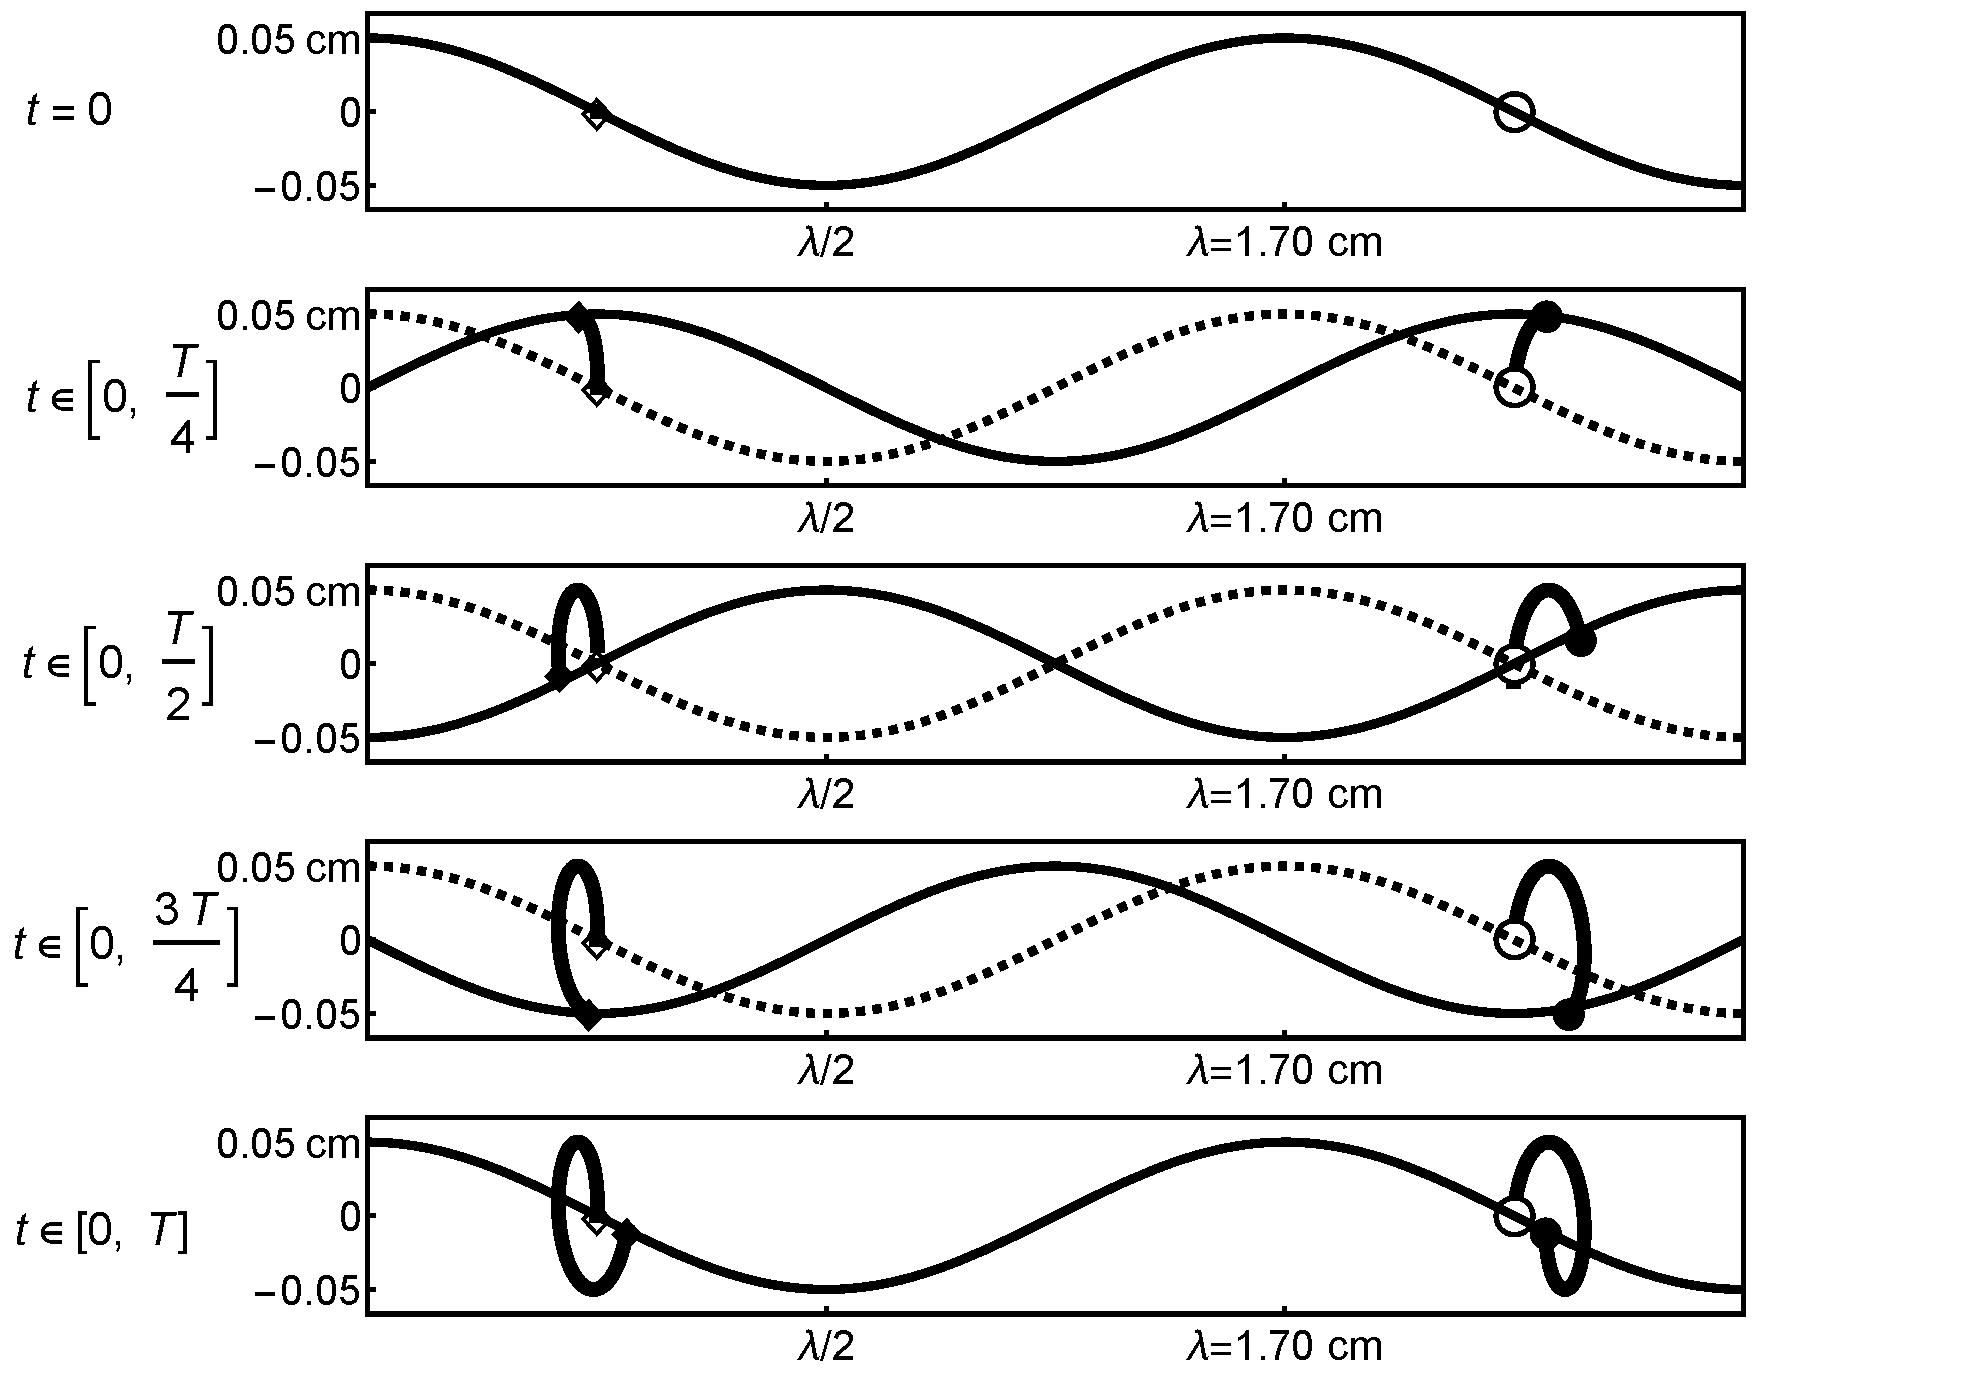
\includegraphics[scale=0.55]{U0}
\caption{Траектории жидких частиц верхней и нижней жидкости при отсутствии поступательного движения верхней среды ($ U_{0}=0 $)}\label{fig:Traj1}
\end{figure}
Графики показывают последовательное смещение жидких частиц с временным интервалом $ \Delta T = T/4 $, соответствующим четверти периода волнового движения. Видно, что в отсутствии относительного движения сред, жидкие частицы совершают петлеобразные движения во встречных направлениях. А обе частицы с течением времени смещаются в направлении распространения волны с одинаковой средней дрейфовой скоростью (см.~\eqref{UdriftNizh} и~\eqref{UdriftVerh}).

На рисунке~\ref{fig:Traj2} демонстрируется траектория жидкой частицы нижней жидкости за 29 периодов волнового движения. 
\begin{figure}[ht]
\centering
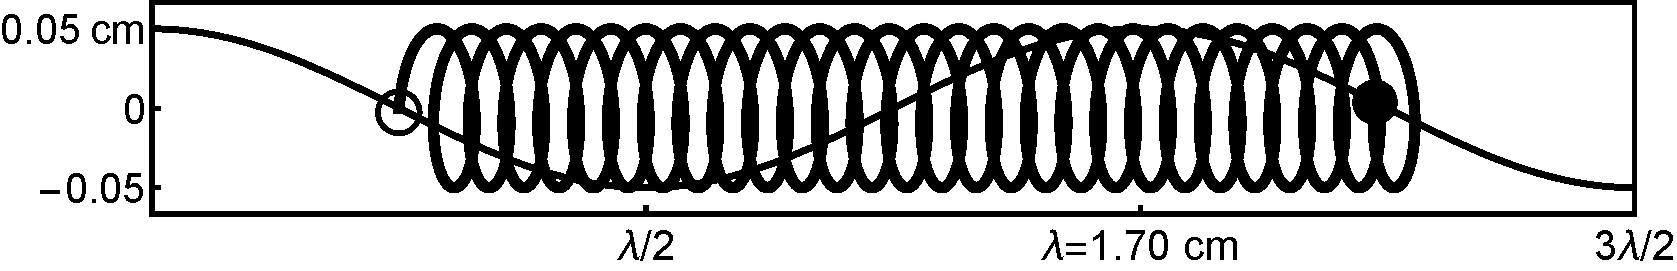
\includegraphics[scale=0.6]{U50_nizh}
\caption{Траектория движения частиц нижней жидкости за время, необходимое для дрейфа на расстояние порядка длины волны.}\label{fig:Traj2}
\end{figure}
Из~\eqref{Period} следует, что $ t_{\lambda}/T\perm=\zeta^{-2}k^{-2}\perm\approx 29.4 $ доля в периодах волнового движения, необходимая для дрейфа на расстояние соответствующее длине волны. Рисунок~\ref{fig:Traj2} останется неизменным при увеличении скорости $ U_{0} $ до критического значения $ U_{cr}\approx 730\, \text{см/сек} $ при измерении времени в долях волнового периода, а не в абсолютных значениях.

Рисунок~\ref{fig:Traj3} построен для значения скорости сдвигового движения верхней жидкости $ U_{0}=10\, \text{см/сек} $. 
\begin{figure}[!h]
\centering
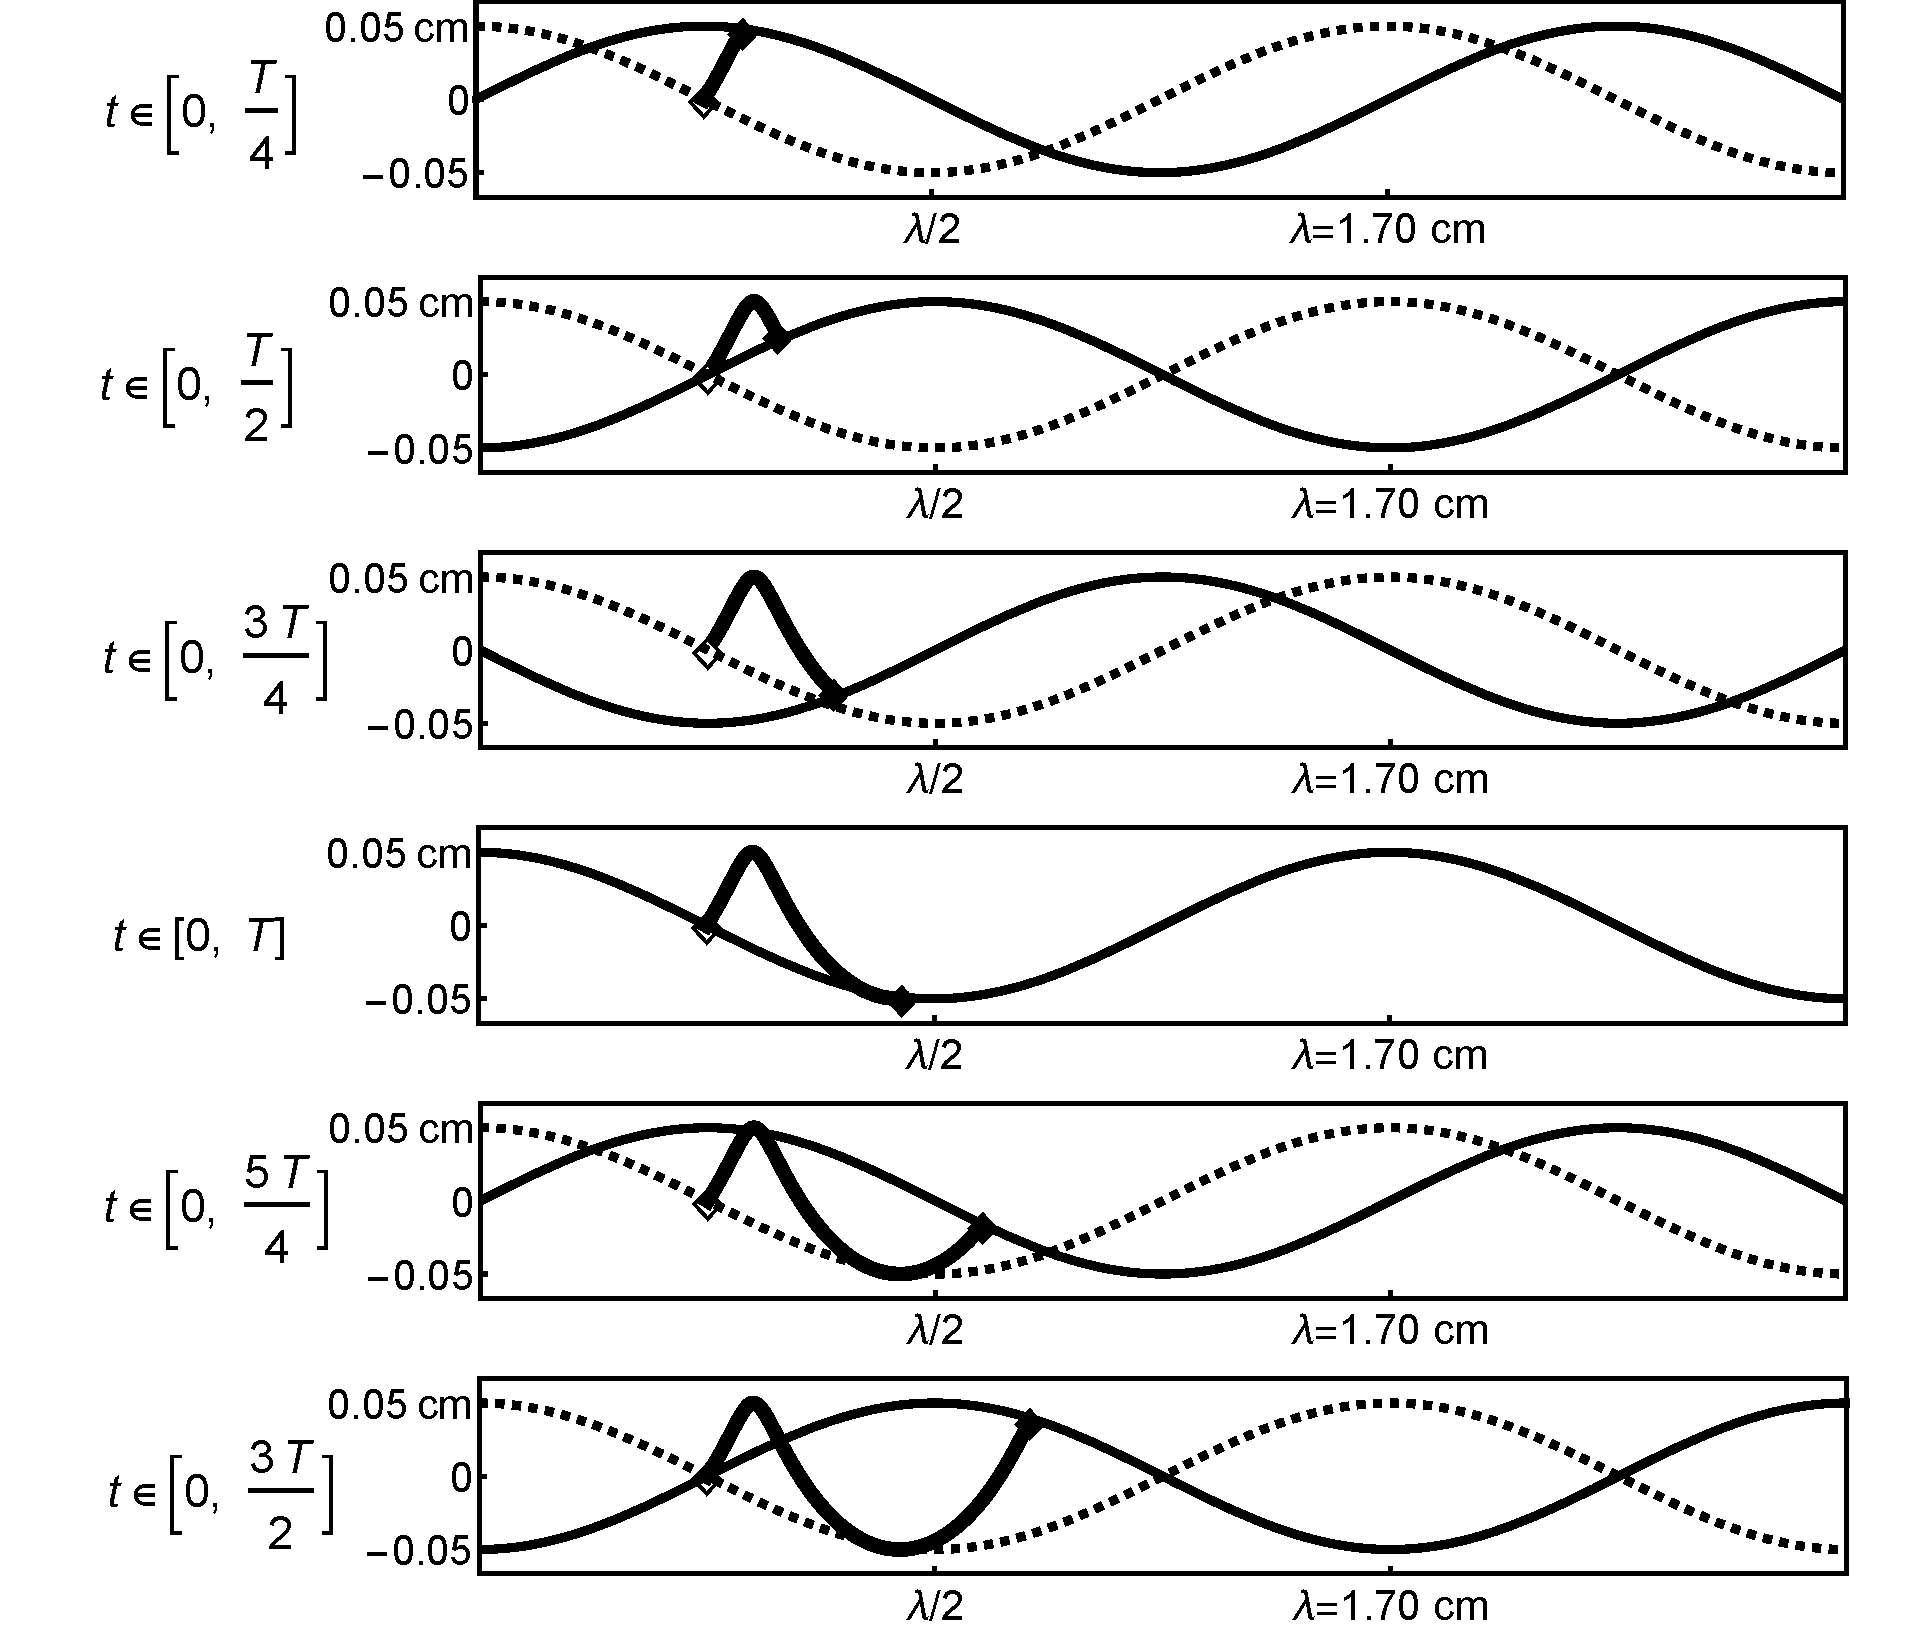
\includegraphics[scale=0.55]{U10}
\caption{Траектории движения частиц верхней среды при значении $ U_{0}=10 $~см/сек в неподвижной лабораторной системе отсчета.}\label{fig:Traj3}
\end{figure}
Из рисунка~\ref{fig:Traj3} видно, что даже такая небольшая скорость сдвига вносит существенные изменения в форму траекторий движения частичек верхней среды: петлеобразное движение трансформируется в дугообразное с заметным смещением в направлении движения среды. И при выполнении условия $ U_{0}<U_{ph} $ жидкая частица за период волнового движения смещается на расстояние меньшее, чем длина волны, а дрейфовая добавка сонаправлена с направлением поступательного движения верхней среды. На рисунке~\ref{fig:Traj4} представлено как выглядит траектория движения той же самой жидкой частицы, но в системе отсчета, движущейся совместно со всей массой верхней жидкости со скоростью $ U_{0}=10\, \text{см/сек} $. 
\begin{figure}[ht]
\centering
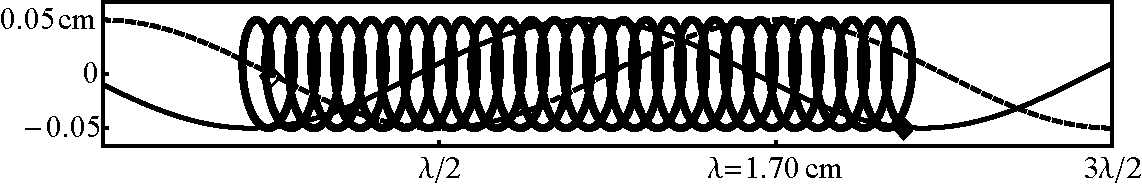
\includegraphics[scale=0.9]{U10UAir}
\caption{Траектории движения частиц верхней среды при значении $ U_{0}=10 \, \text{см/сек}<U_{ph}$ в системе отсчета, связанной с верхней средой за время, необходмое для дрейфа на расстояние порядка длины волны в этой системе отсчета.}\label{fig:Traj4}
\end{figure}
Траектория построена за 2 периода волнового движения , поскольку из~\eqref{Period'} следует, что доля, волновых периодов, необходимая для дрейфа жидкой частички на расстояние равное длине волны $ t'_{\lambda}/T=1/\left( \beta+\zeta^{2}k^{2}\left( 1-\beta \right) \right) \approx 2.2 $. Траектории, аналогичные представленным на рисунке~\ref{fig:Traj3} и рисунке~\ref{fig:Traj4} будут наблюдаться у жидких частичек верхней жидкости при условии, когда скорость относительного сдвига не достигает фазовой скорости волнового движения $ 0<U_{0}<U_{ph} $.
Дальнейший рост $ U_{0} $ приводит к уменьшению модуля дрейфовой добавки и при достижении фазовой скорости $ U_{0}=U_{ph} $ добавка принимает нулевое значение, а период круговых движений жидкой частички стремится к бесконечному значению. Что соответствует равномерному и прямолинейному движению жидких частиц с фазовой скоростью волны $ U_{0}=U_{ph}\approx 23 \, \text{см/сек} $ (рисунок~\ref{fig:Traj5}). В системе отсчета движущейся в том же направлении с фазовой скоростью жидкие частицы верхней жидкости оказываются покоящимися.
\begin{figure}[ht]
\centering
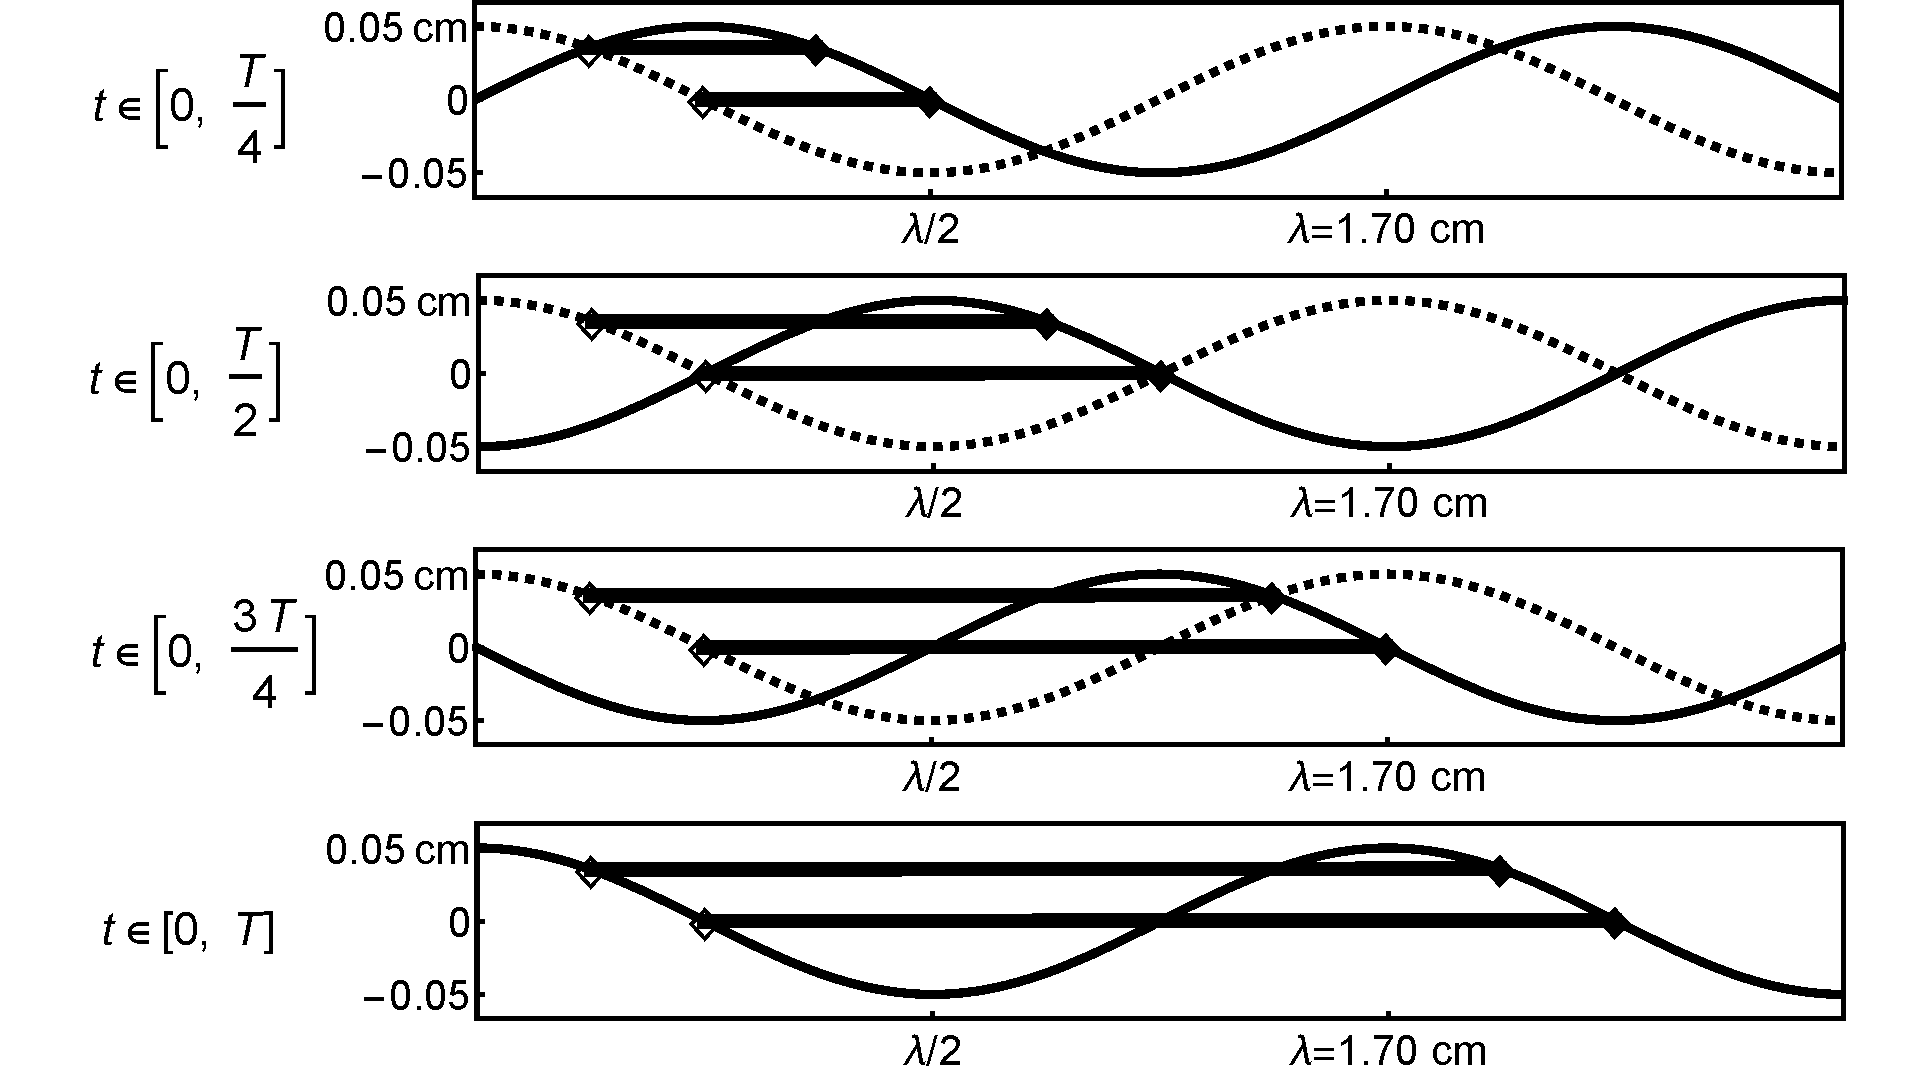
\includegraphics[scale=0.55]{U23}
\caption{Траектории движения частиц верхней среды при значении $ U_{0}=23\, \text{см/сек}\simeq U_{ph}$ в неподвижной лабораторной системе отсчета.}\label{fig:Traj5}
\end{figure}
 
На рисунке~\ref{fig:Traj6} проиллюстрирована траектория движения жидкой частички верхней среды при скорости сдвига $ U_{0}=50\, \text{см/сек} $. Частица движется по сильно вытянутой дугообразной траектории, и за период волнового движения перемещается на расстояние, превышающее длину волны. Дрейфовая добавка при этом направлена в сторону, противоположную поступательному движению верхней среды и увеличивается с увеличением $ U_{0} $. 
\begin{figure}[ht]
\centering
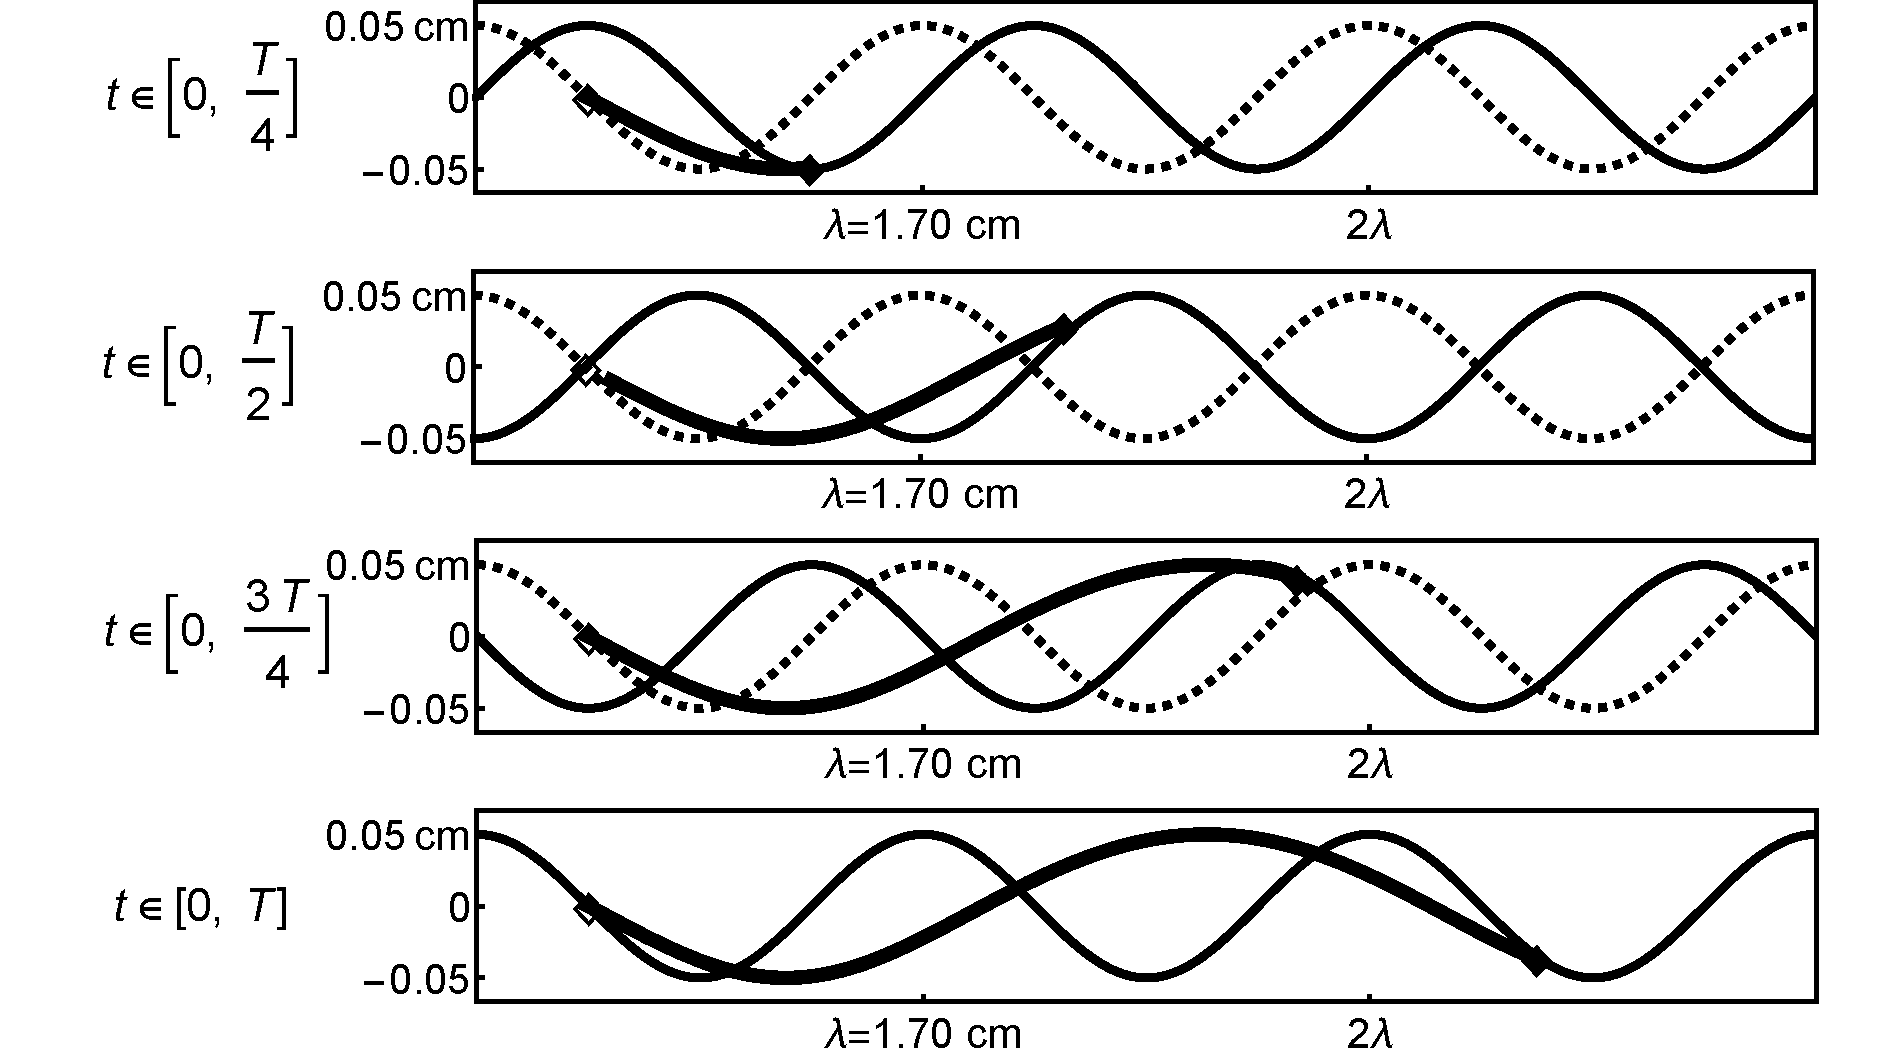
\includegraphics[scale=0.55]{U50}
\caption{Траектории движения частиц верхней среды при значении $ U_{0}=50\, \text{см/сек}>U_{ph} $ в неподвижной лабораторной системе отсчета.}\label{fig:Traj6}
\end{figure}
На рисунке~\ref{fig:Traj7} показана траектория движения жидкой частички из системы отсчета, движущейся вправо со скоростью относительного сдвига $ U_{0}=50\, \text{см/сек} $. При таком значении скорости $ U_{0} $ доля периода волнового движения необходимая для дрейфа на расстояние равное длине волны $ t'_{\lambda}/T=1/\left( \beta+\zeta^{2}k^{2}\left( 1-\beta \right) \right) \approx 0.5 $. 
\begin{figure}[ht]
\centering
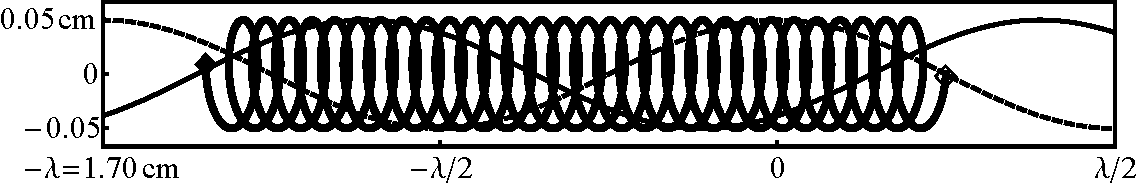
\includegraphics[scale=0.8]{U50UAir}
\caption{Траектории движения частиц верхней среды при значении $ U_{0}=50\, \text{см/сек}>U_{ph} $ в системе отсчета, связанной с верхней средой.}\label{fig:Traj7}
\end{figure}
Подобная картина будет наблюдаться для всех значений скорости $ U_{0} $ при выполнении неравенства $ U_{ph}<U_{0}<U_{cr} $.


\newpage
\subsection{Область закритических значений в смысле реализации неустойчивости Кельвина--Гельмгольца}
\label{Sec:Zacr}

Если скорость поступательного движения верхней среды превышает критическое значение в смысле реализации неустойчивости Кельвина--Гельмгольца ($ U_{0}>U_{cr} $ ), то поверхность раздела дестабилизируется. При этом частота волнового движения  принимает комплексные значения. Действительная часть круговой частоты при этом описывается выражением:
\begin{equation*}
\sigma = Re\left( \omega \right)= \dfrac{k \rho' U_{0}}{\rho+\rho'}, 
\end{equation*}
а мнимая часть записывается:
\begin{equation*}
r=Im \left( \omega \right)=\dfrac{\sqrt{k^{2}\rho \rho' U^{2}_{0}-k g \left( \rho^{2}-\rho'^{2} \right) -k^{3} \gamma \left( \rho+\rho' \right)}}{\rho+\rho'}.
\end{equation*}

Мнимая составляющая принимает положительные значения для одного из корней дисперсионного уравнения и отрицательные для другого. Значение $ r>0 $  характеризует инкремент нарастания неустойчивости Кельвина--Гельмгольца, связанной с волновым возмущением границы раздела с волновым числом $ k $. Корень с таким значением параметра $ r $ представляет интерес для рассмотрения в настоящей работе.

На начальном этапе развития неустойчивости поле скоростей~---  модифицируется. В нижней жидкости скорости выглядят следующим образом:
\begin{equation*}
u_{1}=\dfrac{1}{2}\zeta \sigma \exp \left( i \left( \sigma t - k x\right) \right) \exp \left( k z \right) \exp \left( r t\right) +C.C.
\end{equation*}
\begin{equation*}
v_{1}=-\dfrac{i}{2}\zeta \sigma \exp \left( i \left( \sigma t - k x\right) \right) \exp \left( k z \right) \exp \left( r t\right) +C.C.
\end{equation*}
	
Поле скоростей в верхней жидкости опишется соотношениями:
\begin{equation*}
u'_{1}=U_{0}-\dfrac{1}{2}\zeta \left( \sigma-k U_{0}\right) \exp \left( i \left( \sigma t - k x\right) \right) \exp \left(- k z \right) \exp \left( r t\right) +C.C.
\end{equation*}
\begin{equation*}
v'_{1}=\dfrac{i}{2}\zeta \left( \sigma-k U_{0}\right) \exp \left( i \left( \sigma t - k x\right) \right) \exp \left(- k z \right) \exp \left( r t\right) +C.C.
\end{equation*}
	
Производя преобразования, аналогичные описанным в предыдущих пунктах получаем скорость дрейфового движения в нижней и верхней жидкостях при $ U_{0}>U_{cr} $:
\begin{equation*}
U_{DS}=\zeta^{2}\sigma k \exp \left( 2 r t\right) \exp \left( 2 k z \right)
\end{equation*}
\begin{equation*}
U'_{DS}=U_{0}+\zeta^{2} \left( \sigma-k U_{0} \right) k \exp \left( 2 r t\right) \exp \left( -2 k z \right)
\end{equation*}

Дрейфовые добавки  направлены в противоположные стороны и экспоненциально нарастают со временем, что должно приводить к уменьшению тангенциального разрыва скоростей, и как следствие, к стабилизации поверхности. 

\section{Заключение}

Разработана аналитическая асимптотическая для расчета лагранжевой скорости и траекторий движения материальных частиц, участвующих в волновом движении, связанным с возмущением горизонтальной границы раздела двух несмешивающихся идеальных жидкостей. Модель эффективно описывает влияние относительного горизонтального перемещения сред на динамику индивидуального и коллективного движения жидких частиц. 

Обнаружено новое свойство неустойчивости Кельвина--Гельмгольца. Даже в модели идеальной жидкости помимо экспоненциального нарастания амплитуды изначально малых возмущений границы раздела существует стабилизирующий механизм. Он проявляется в экспоненциальном росте дрейфовых течений в обеих средах, направленных таким образом, чтобы уменьшить тангенциальный скачок скоростей, инициировавший неустойчивость.